\documentclass[10pt,journal,letter,compsoc]{IEEEtran}
\usepackage{booktabs}
\usepackage{tabularx}
\usepackage[english]{babel}
\usepackage[ruled]{algorithm}
\usepackage{algpseudocode}
\usepackage{color}
\usepackage{enumitem}
\let\proof\relax
\let\endproof\relax 
\usepackage{amsthm}
\usepackage[cmex10]{amsmath}
\usepackage{amsfonts}
\usepackage{multicol}
\let\subcaption\relax
\usepackage[font=small]{subcaption}
\usepackage{graphicx}
\usepackage[hidelinks,bookmarks=false,pdfpagelabels]{hyperref}
\usepackage[nocompress]{cite}

%\special{papersize=8.5in,11in}
%\setlength{\pdfpageheight}{\paperheight}
%\setlength{\pdfpagewidth}{\paperwidth}

% definition environment
\newtheorem{definition}{Definition}
\newtheorem{theorem}{Theorem}
\newtheorem{lemma}{Lemma}
\newtheorem{invariant}{Invariant}

% typewriter font family that support hyphenation
%\newcommand\textvtt[1]{{\normalfont\fontfamily{cmvtt}\selectfont #1}}
\hyphenation{MD-List} 
\hyphenation{skip-list}
\hyphenation{De-le-te-Min}

\algtext*{EndWhile}
\algtext*{EndFor}
\algtext*{EndIf}
\algtext*{EndFunction}
\newcommand\NIL{\text{NIL}}
\newcommand\TRUE{\text{\textbf{true}}}
\newcommand\FALSE{\text{\textbf{false}}}
\newcommand\BREAK{\text{\textbf{break}}}
\newcommand\CONTINUE{\text{\textbf{continue}}}
\newcommand\AND{\;\text{\textbf{and}}\;}
\newcommand\OR{\;\text{\textbf{or}}\;}
\algrenewcommand\algorithmicindent{1em}

\algblockdefx[StructBlock]{Struct}{EndStruct} [1]{\textbf{struct} #1} [0]{}
\algtext*{EndStruct}
\algblockdefx[ClassBlock]{Class}{EndClass} [1]{\textbf{class} #1} [0]{}
\algtext*{EndClass}
\algblockdefx[MacroBlock]{Define}{EndDefine} [2]{\textbf{define} #1(#2)} [0]{}
\algtext*{EndDefine}
\algblockdefx[InlineBlock]{Inline}{EndInline} [2]{\textbf{inline function} \textsc{#1}(#2)} [0]{}
\algtext*{EndInline}

\begin{document}

\title{A Lock-free Priority Queue Design Based on Multi-dimensional Linked Lists}
%\authorinfo{Deli Zhang\and Damian Dechev}{University of Central Florida}{de-li.zhang@knights.ucf.edu\and dechev@eecs.ucf.edu}

\author{Deli~Zhang and~Damian~Dechev%
\IEEEcompsocitemizethanks{\IEEEcompsocthanksitem The authors are with the Department of Electrical Engineering and Computer Science, University of Central Florida, Orlando, FL, 32826. \protect\\
E-mail: de-li.zhang@knights.ucf.edu and dechev@eecs.ucf.edu}}

\IEEEtitleabstractindextext{
\begin{abstract}
    The throughput of concurrent priority queues is pivotal to multiprocessor applications such as discrete event simulation, best-first search and task scheduling. 
    Existing lock-free priority queues are mostly based on skiplists, which probabilistically create shortcuts in an ordered list for fast insertion of elements.
    The use of skiplists eliminates the need of global rebalancing in balanced search trees and ensures logarithmic sequential search time on average, but the worst-case performance is linear with respect to the input size.
    In this paper, we propose a quiescently consistent lock-free priority queue based on a multi-dimensional list that guarantees worst-case search time of $\mathcal{O}(\log N)$ for key universe of size $N$.
    The novel multi-dimensional list (MDList) is composed of nodes that contain multiple links to child nodes arranged by their dimensionality. 
    The insertion operation works by first injectively mapping the scalar key to a high-dimensional vector, then uniquely locating the target position by using the vector as coordinates.
    Nodes in MDList are ordered by their coordinate prefixes and the ordering property of the data structure is readily maintained during insertion without rebalancing nor randomization.
    In our experimental evaluation using a micro-benchmark, our priority queue achieves an average of $50\%$ speedup over the state of the art approaches under high concurrency.
\end{abstract}

%\category{D.1.3}{Concurrent Programming}{Algorithms}
%\terms{Algorithms, Performance}
\begin{IEEEkeywords}
    Concurrent Data Structure, Priority Queue, Lock-freedom, Multi-dimensional List, Skiplist
\end{IEEEkeywords}
}
\maketitle

\IEEEraisesectionheading{\section{Introduction}}
\IEEEPARstart{S}{calable} non-blocking priority queues are pivotal to the performance of parallel applications on current multi-core and future many-core systems.
Attempts on parallelizing search algorithms, such as best-first search~\cite{burns2010best}, do not achieve the desired performance gains due to the lack of scalable concurrent priority queues.
Priority task scheduling~\cite{wimmer2013data} and discrete event simulation applications~\cite{linden2013skiplist} also demand high-throughput priority queues to efficiently distribute workload.
A priority queues is an abstract data structure that stores a set of key-value pairs where the keys are totally ordered and interpreted as priorities. 
A priority queue is defined only by its semantics that specify two canonical operations: \textsc{Insert}, which adds a key-value pair, and \textsc{DeleteMin}, which returns the value associated with the key of highest priority and removes the pair from the queue.
In sequential execution scenarios, priority queues can be implemented on top of balanced search trees or array-based binary heaps~\cite{cormen2001introduction}. 
The latter is more efficient in practice because its compact memory footprint exploits spatial locality that optimizes cache utilization. 
For concurrent accesses by a large number of threads balanced search trees suffer from sequential bottlenecks due to required global rebalancing.
Array-based heaps suffer from heavy memory contention in the heapify operation when a newly inserted key ascends to its target location.

In recent research studies~\cite{linden2013skiplist,sundell2005fast,herlihy2006provably,fraser2007concurrent}, concurrent priority queue algorithms based on skiplists are gaining momentum.
A skiplist~\cite{pugh1990skip} is a linked list that provides a probabilistic alternative to search trees with logarithmic sequential search time on average. 
It eliminates the need of rebalancing by using several linked lists, organized into multiple levels, where each list skips a few elements. 
Links in the upper levels are created with exponentially smaller probability.
Due to the nature of randomization, skiplists still exhibit less than ideal linear worst-case search time.
Skiplist-based concurrent priority queues have a distributed memory structure that allows concurrent accesses to different parts of the data structure efficiently with low contention. 
However, \textsc{Insert} operations on skiplists involve updating shortcut links in distant nodes, which incurs unnecessary data dependencies among concurrent operations and limits the overall throughput.
Another bottleneck faced by concurrent priority queues is the inherent sequential semantics required by the \textsc{DeleteMin} operation~\cite{ellen2012inherent}.
Threads competing to remove the minimal element from the queue squander most of their effort trying to decide which one gets the minimal node.
The best existing approach employs logical deletion and batch physical deletion to alleviate the contention on head nodes~\cite{linden2013skiplist}, but the parallelism achieved by this approach is still limited because threads performing deletion have to traverse all logically deleted nodes and are forced to wait for slow insertions.
%Semantics relaxation~\cite{henzinger2013quantitative} opens up an opportunity to trade strict correctness guarantees, such as linearizability~\cite{herlihy1990linearizability}, for better throughput.

In this paper, we present a quiescently consistent lock-free priority queue design based on a multi-dimensional list (MDList).
The proposed multi-dimensional list stores ordered key-value pairs and guarantees worst-case sequential search time of $\mathcal{O}(\log N)$ where $N$ is the size of the key universe.
It is composed of nodes that contain multiple links to the child nodes arranged by their dimensionality, and provides convenient concurrent accesses to different parts of the data structure.
The insertion works by first injectively mapping a scalar key into a high dimensional vector, then uniquely locating the target position using the vector as coordinates.
Similar to a trie data structure~\cite{willard1983log}, a node in MDList shares the same coordinate prefix with all of its parent nodes, and the search is done through prefix matching rather than key comparison.
As a result, the ordering property of the data structure is readily maintained during insertion without rebalancing nor randomization.
The proposed priority queue satisfies lock-freedom, which ensures system wide progress while allowing individual threads to starve~\cite{herlihy2012art}.
It has the following algorithmic characteristics that aim to further improve the throughput over existing approaches by exploiting a greater level of parallelism and reducing contention among concurrent operations.

\begin{itemize}
    \item Each insertion modifies at most two consecutive nodes, which allows concurrent insertions to be executed with minimal interference.
    \item A \emph{deletion stack} is used to provide hints about the next minimum node so that \textsc{DeleteMin} operations do not need to traverse logically deleted nodes.
    \item Insertions proceed optimistically without blocking overlapping deletions; they synchronize with \textsc{DeleteMin} operations only when necessary by rewinding the deletion stack.
\end{itemize}

In our experimental evaluation, we compare our algorithm with Intel TBB's priority queue and the best available skiplist-based priority queues using a micro-benchmark on a 64-core NUMA and a 12-core SMP system for three types of workload. 
The result shows that on the NUMA system our algorithm outperforms the alternative approaches by an average of $50\%$ under high concurrency.
On the SMP system, our algorithm achieves the same level of performance as the best skiplist-based approach for mixed workload and outperforms the alternatives for insert-only workload. 
We also show that the dimensionality of an MDList-based priority queue can be tuned to fit different workloads.

The rest of the paper is organized as follows. 
In Section~\ref{sec:related}, we review existing concurrent priority queue algorithms.
In Section~\ref{sec:mdlist}, we define the multi-dimensional list data structure and introduce the sequential search algorithm.
We present the concurrent \textsc{Insert} and \textsc{DeleteMin} operations for our MDList-based lock-free priority queue in Section~\ref{sec:cpqueue}.
We reason about its correctness and progress properties in Section~\ref{sec:correctness}.
The performance evaluation and result analysis is given in Section~\ref{sec:experiment}.
We conclude the paper in Section~\ref{sec:conclusion}.

%\vspace{-0.2in}
\section{Related Work}
\label{sec:related}
As a fundamental data structure, concurrent priority queues have been extensively studied in the literature.
Early concurrent priority queue algorithms are mostly adaptations of the sequential heap data structure.
Hunt et al.~\cite{hunt1996efficient} present a fine-grained locking approach that is built on a number of earlier heap-based algorithms.
Herlihy~\cite{herlihy1993methodology} uses an array-based binary heap as an example for the universal construction of lock-free data structures.
It requires that each thread only modify a local copy of the heap and updates the pointer to the heap using atomic operations.
This serves as a fault tolerance scheme to avoid deadlocks rather than exploit fine-grained parallelism.
Both of these approaches, like all heap-based algorithms, suffer from sequential bottlenecks and contention due to the compact memory layout of the data structure.
We omit detailed discussion on more heap-based approaches as empirical evidence collected on modern multi-core platforms shows that they are outperformed by recent skiplist-based structures~\cite{shavit2000skiplist,sundell2005fast}.

Pugh~\cite{pugh1990concurrent} designs a concurrent skiplist with per-pointer locks, where an update to a pointer must be protected by a lock. 
Shavit~\cite{shavit1999scalable} discovers that the highly decentralized skiplist is suitable for shared-memory systems and presents a bounded priority queue based on Pugh's algorithm using fixed bins. 
However, this approach only supports a small set of fixed priorities whereas our approach supports an arbitrary range of keys.
Shavit and Lotan~\cite{shavit2000skiplist} also propose the first unbounded concurrent priority queue based on a skiplist.
Their locking approach employs logical deletion (by marking the target) that kept a specialized pointer to the current minimal item, and each \textsc{DeleteMin} operation has to traverse the lowest level list until it finds an unmarked item.
A lock-free adaptation of this algorithm was later presented by Herlihy and Shavit~\cite{herlihy2012art}.
Sundell and Tsigas~\cite{sundell2005fast} present the first linearizable lock-free priority queue based on a skiplist.
They guarantee linearizability by forcing threads to help physically remove a node before moving past it.
Herlihy et al.~\cite{herlihy2006provably} propose an optimistic concurrent skiplist that simplifies previous work and allows for easy proof of correctness while maintaining comparable performance.
Recently, Linden and Jonsson~\cite{linden2013skiplist} propose a skiplist-based lock-free priority queue that addresses the sequential bottleneck of the \textsc{DeleteMin} operation.
Their design uses a logical deletion scheme similar to Shavit and Lotan's approach described above, but provides significant performance improvement by performing physical deletions in batch. 
The drawback was that the logically deleted nodes have to always form a prefix of the lowest level list, and physical deletions cannot pass ongoing insertions.

As recognized by the above researches, the \textsc{DeleteMin} operation presents the biggest scalability challenge for concurrent priority queues.
Concurrent data structures that are strictly adherent to linearizability often pay a price for performance and scalability.
Relaxed semantics for concurrent data structures are proposed to provide considerable performance benefit when tight synchronization is not absolutely necessary~\cite{afek2010quasi,henzinger2013quantitative}.
Henzinger et al.~\cite{henzinger2013quantitative} proposed a formalization of semantics relaxation for concurrent priority queues.
Alistarh et al.~\cite{alistarh2014spraylist} present a relaxed algorithm by allowing deletion threads to randomly pick a node within a certain priority range.
Wimmer et al.~\cite{wimmer2013data} study the performance of semantically relaxed priority queues for task scheduling.
%Liu and Spear~\cite{liu2012mounds} proposed a concurrent priority queue based on a hybrid data structure called the mound.
%Their approach consists of a rooted tree of sorted linked lists, which supports simultaneously extract multiple elements from the head of the queue.
%However, their lock-free implementation requires double-word CompareAndSwap, and relies on randomization to balance the length of each sub-lists.
While the above approaches study the trade-offs of semantic relaxation, this paper tries to exploit the performance benefit of relaxing the consistency criteria.

The proposed MDList also bears some similarity to trie data structures~\cite{fredkin1960trie,willard1983log} in that the keys are ordered by their prefixes: a node always shares the same key prefix with its parent nodes.
Lock-free trie designs such as the concurrent tries~\cite{prokopec2012concurrent} and the skiptrie~\cite{oshman2013skiptrie} provides log-logarithm search time, but their algorithm cannot be readily transfered to a priority queue implementation.
%To the best of our knowledge, there is no lock-free implementation of priority queue based on a regular trie data structure. 
One difficulty is that the minimum item in a trie is stored in a leaf node, so its retrieval has to be done through repetitive search.
Designing linearizable \textsc{DeleteMin} is also challenging in a trie, because new minimum items can be concurrently inserted at higher level while the \textsc{DeleteMin} operation proceeds to lower levels.
MDList, on the other hand, behaves like a heap where the root node always holds the item with the smallest key.

%TODO: performance trade-off related, include it only when page limit allows
%Fraser and Harris outline the design of three concurrent skip lists using CAS, MCAS, and FSTM~\cite{fraser2007concurrent}.
%They illustrate the trade-off between simplicity and efficiency among these implementations: CAS-base skip lists provides superior performance over the other two, and the FSTM-based approach is straightforward to implement; MCAS-based approach reaches for the middle ground between the former two methods.

\section{Multi-dimensional List}
\label{sec:mdlist}
The core idea of a multi-dimensional list is to partition a linked list into shorter lists and rearrange them in a multi-dimensional space to facilitate search.
Just like a point in a $D$-dimensional space, a node in a $D$-dimensional list can be located by a $D$-dimensional coordinate vector.
The search operation examines one coordinate at a time and locates correspondent partitions by traversing nodes that belong to each dimension. 
The search time is bounded by the dimensionality of the data structure and logarithmic time is achieved by choosing $D$ to be a logarithm of the key range. 
%We limit our discussion on three operations search, insertion and deletion which is needed by priority queues, but it is possible to support other operations as well.

\vspace{-0.09in}
\subsection{From Linked List to 2DList}
\label{sec:mdlist-overview}
An ordered linked list keeps its nodes sorted linearly as if they were attached to a one-dimensional line.
To find an existing node or insert a new node, one starts from the head and examines each node consecutively.
The search time is linear with respect to the list capacity.
The linked list illustrated in Fig.~\ref{fig:mdlist1d} has 16 nodes partitioned into 4 columns. 
This arrangement reveals a property concealed by the typical one-dimensional representation: the nodes are sorted along the columns as well as across the rows, and each column contains a unique range of nodes that have greater keys than the nodes in the previous column.
Because a column is substantially shorter than the entire list, we can locate a node much faster if we firstly determine which column the node resides, and search for it within the column. 
However, a one-dimensional linked list lacks two essential properties required by the above search scheme: 1) short-cut links among columns which allow the search operation to switch from one column to another; 2) a function that maps keys into key ranges covered by each column.

\vspace{-0.05in}
\begin{figure}[h]
    \begin{subfigure}{0.48\columnwidth}
        \centering
        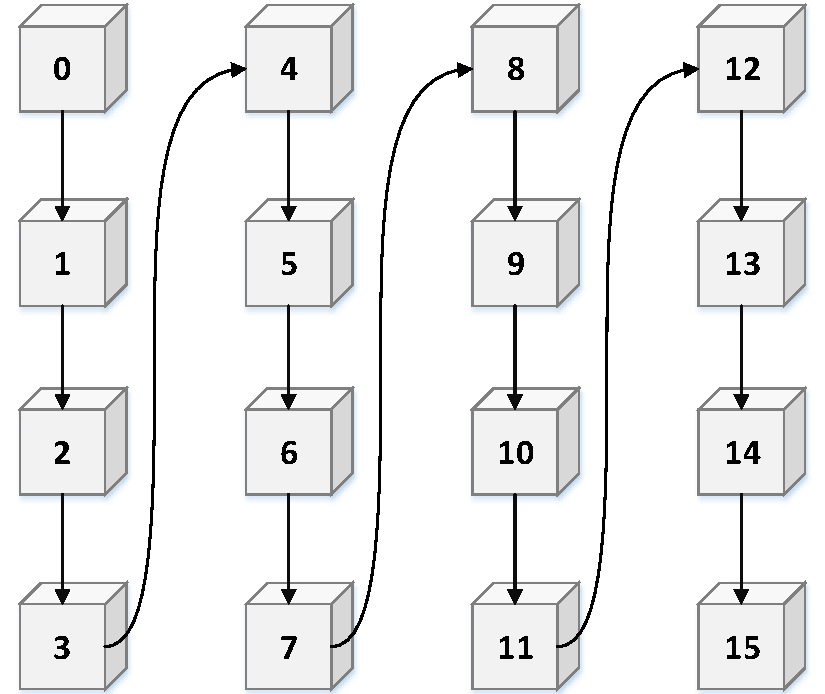
\includegraphics[width=1\columnwidth]{./graph/mdlist-1d}
        \caption{Linked List}
        \label{fig:mdlist1d}
    \end{subfigure}
    \hfill
    \begin{subfigure}{0.48\columnwidth}
        \centering
        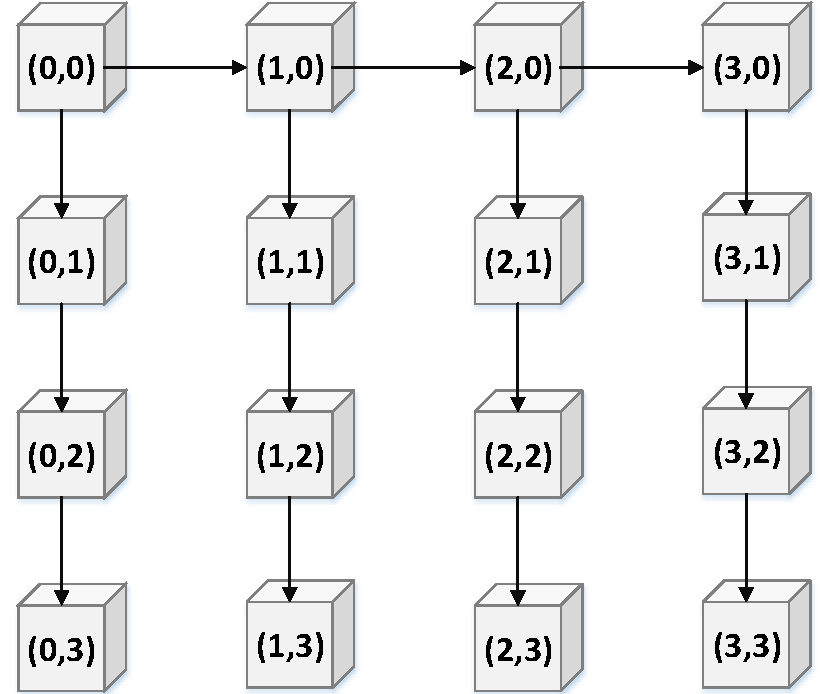
\includegraphics[width=1\columnwidth]{./graph/mdlist-2d}
        \caption{2DList}
        \label{fig:mdlist2d}
    \end{subfigure}
    \caption{From linked list to 2DList}
    \label{fig:mdlist}
\end{figure}
\vspace{-0.1in}

We show a sample construction of a 2DList that satisfies these requirements in Fig.~\ref{fig:mdlist2d}.
We replace the pointers linking the bottom nodes to the top nodes in Fig.~\ref{fig:mdlist1d} by links among the top nodes so that the top of each column form a one-dimensional linked list.
This essentially converts the linked list into a tree, but we find it more intuitive to visualize it as a multi-dimensional list when discussing the algorithms in the following sections.
We also compute a 2-dimensional vector $\mathbf{k}=(k_0,k_1)$ based on the integer key, which serves as a node's unique coordinates in the 2-dimensional space.
We discuss the mapping from integer keys to vectors in more detail in Section~\ref{sec:coord}.
The nodes are arranged such that the top nodes of each column are ordered by $k_0$, while every node in one column shares the same $k_0$ and is ordered by $k_1$.
We call the top nodes \emph{dimension 0 nodes} (because they are ordered by the 0th element in the coordinate vector), and the nodes in each column \emph{dimension 1 nodes}.
To search for a node, for example $(2,3)$, we begin by traversing the dimension 0 nodes as if we were traversing a one-dimension linked list.
The difference is that instead of examining the actual key we examine the $k_0$ of each node and compare it against the target's $k_0$.
We stop at node $(2,0)$, and continue to traverse the third column, which consists of dimension 1 nodes. 
We look for the node with $k_1 = 3$ and eventually locate the target.
The average and worst-case search times are reduced to a square root of the original times, and we can further improve them by extending the 2DList into higher dimensions.

\vspace{-0.05in}
\theoremstyle{definition}
\subsection{Definition}
We generalize the construction of the 2DList to a list of arbitrary dimensions and give the following definition of our multi-dimensional list.
\vspace{-0.05in}
\begin{definition}
\label{def:mdlist}
A $D$-dimensional list is a rooted tree in which each node is implicitly assigned a dimension of $d \in [0,D)$. The root node's dimension is $0$. A node of dimension $d$ has no more than $D-d$ children, and each child is assigned a unique dimension of $d' \in [d,D)$. 
\end{definition}
\vspace{-0.05in}

In an ordered multi-dimensional list, we associate every node with a coordinate vector $\mathbf{k}$, and determine the order among nodes lexicographically based on $\mathbf{k}$.
A dimension $d$ node should share a coordinate prefix of length $d$ with its parent.
The following requirement prescribes the exact arrangement of nodes according to their coordinates.
%and sort the dimension $d$ nodes according to $k_d$ as depicted in Fig.~\ref{fig:mdlist2d}.

\vspace{-0.05in}
\theoremstyle{definition}
\begin{definition}
\label{def:mdlistsort}
    Given a non-root node of dimension $d$ with coordinate $\mathbf{k}=(k_0,...,k_{D-1})$ and its parent with coordinate $\mathbf{k'}=(k'_0,...,k'_{D-1})$ in an ordered $D$-dimensional list: $k_i = k'_i, \;\forall \;i \in [0, d) \land k_d > k'_d$.
\end{definition}
\vspace{-0.05in}

A fundamental property is that a high-dimensional list can be decomposed into low-dimensional lists: every dimension 0 node in a $D$-dimensional list can be seen as the root node of a $(D-1)$-dimensional list.
If we repeat the decomposition process recursively, we obtain multi-dimensional lists with fewer and fewer dimensions and eventually we arrive at a single node.
This is analogous to affine subspaces, or flats, in a $\mathbb{Z}_{\ge 0}^D$-affine space.
The design of the search algorithm detailed in Section~\ref{sec:search}, is based on prefix traveling the of the affine space.
%This is analogous to the process of slicing a cube into planes and a plane into lines.
%For example, the 2DList in Fig.~\ref{fig:mdlist2d} consists of four 1DLists.

%\begin{theorem}
%\label{def:mdlistsublist}
%In an ordered $D$-dimensional list, all nodes that share the same coordinate prefix (the sequence of coordinates starting from the first coordinate) form an ordered $(D-i)$-dimensional list, where $i$ is the length of the prefix.
%\end{theorem}

%\begin{proof}
    %Let $S$ be the set of nodes that share the coordinate prefix $\mathbf{p}$, $l$ be the $(D-d)$-dimensional list formed by $S$, and $n \in S$ be the root node of $l$. Assume there exists a node $n' \in S$ and $n' \notin l$.
    %with coordinate $\mathbf{k'}$ where $(k'_0,...,k'_d) = \mathbf{p}$.  
%\end{proof}

\vspace{-0.1in}
\subsection{Structures}
We define the structures of a sequential MDList in Algorithm~\ref{alg:structure}. 
The dimension of an MDList is denoted by a constant integer $D$ and the range of the keys by $N$.
The class of MDList itself also contains a pointer to the head (root) node.
The functions presented in the following sections are member functions of the MDList class, which means they have access to the class fields by default.
A node in MDList contains a key-value pair, an array $k[D]$ of integers as the coordinate vector, and an array of child pointers in which the $d$th pointer links to a dimension $d$ child node.
Since nodes of high dimensions have less children than nodes of low dimensions, for a $d$ dimension node it is possible to allocate a child array that fits only $d$ pointers to reduce memory consumption. 
However, for simplicity, we choose to allocate child arrays of size $D$ where $D$ is the dimension of the MDList for all nodes. 
For a dimension $d$ node, only the indices $d$ through $D-1$ of its child array are valid while the rest are unused.
We do not need to store the dimension of a node in the node, it is implicitly deduced by the search algorithm based on the index of the node's pointer in its parent's child array.

\begin{algorithm}[t]
    \caption{MDList Structures}
    \label{alg:structure}
    \vspace{-0.2in}
    \begin{multicols}{2}
        \begin{algorithmic}[1]
            \Class{MDList}
            \State \textbf{const int} $D$
            \State \textbf{const int} $N$
            \State \textbf{Node*} $head$
            \EndClass
            \Struct{Node}
            \State \textbf{int} $key,\;k[D]$
            \State \textbf{void*} $val$
            \State \textbf{Node*} $child[D]$
            \EndStruct
        \end{algorithmic}
    \end{multicols}
    \vspace{-0.15in}
\end{algorithm}

%MDList is more memory efficient than tries and skiplists.
%A regular trie is a d-ary tree with internal nodes and leaf nodes. 
%Values are stored in leaf nodes so pointers to internal nodes consumes extra memory.
%In a skiplist, upper level links are redundant pointers, i.e. a node may have multiple inbound pointers.
%In contrast, an MDList is a not a d-ary tree and every node stores a value.
%Since each node in MDList has exactly one inbound pointer, the memory requirement for MDList is linear with respect to the input size.


%TODO: introduce most significant and least significant coordinate
\subsection{Vector Coordinates}
\label{sec:coord}
There are two requirements for the function that maps a scalar key into a high dimensional vector: 1) it is injective or one-to-one (i.e. distinctness among the keys are preserved); 2) it is monotonic (i.e. the original order among the scalar keys are preserved in the vectors, which are decided by Definition~\ref{def:mdlistsort}).
Additionally, it would be beneficial if the vector coordinates are uniformly distributed so that each dimension of the MDList holds comparable number of nodes. 
Uniform distribution minimizes the number of nodes in each dimension and consequently optimize the search time.
A counter example would be mapping all keys to the first coordinate (i.e. $f(k) \mapsto (k,0,...,0)$), which essential degenerate MDList to a linked list because nodes are not populated to higher dimensions.
There are infinitely many functions that meet the above requirements.
In Algorithm~\ref{alg:mapping}, we present a simple method that uniformly maps integer keys within the range $[0,N)$ into a coordinate vector.

\begin{algorithm}[th]
    \caption{Mapping from integer to vector}
    \label{alg:mapping}
    \begin{algorithmic}[1]
        \Function{KeyToCoord}{$\textbf{int}\;key$}
        \State \textbf{int} $basis \gets \lceil\sqrt[D]{N}\:\rceil,\;quotient\gets key,\;k[D]$
        %\State $basis \gets \lceil\sqrt[D]{N}\:\rceil$
        %\State $quotient \gets key$
        \For {$i \in (D, 0]$}
        \State $k[i] \gets quotient \mod basis$
        \State $quotient \gets \lfloor quotient \div basis \rfloor$
        \EndFor
        \State \Return k
        \EndFunction
    \end{algorithmic}
\end{algorithm}

We first compute the maximum number of nodes in each dimension based on the range of the keys $N$. 
In practice, the range of keys is usually known prior to the execution either explicitly through the user specification of the user application or implicitly through the key's data type.
For example, if the keys are 32-bit integers and we choose the dimension of MDList to be 8, then in each dimension there are at most 16 ($\sqrt[8]{2^{32}}$) keys. 
We can then obtain the coordinate vector by converting the base of the original key. 
In the above case, each digit in the 16-based number corresponds to a coordinate in an 8-dimension vector.
Given a key of 1000, its 16-based representation is \texttt{0x3E8} and the coordinates would be (0,0,0,0,0,3,E,8).
In general, to uniformly distribute keys within range $[0,N)$ in a D-dimension space, the maximum number of keys in each dimension is $b=\lceil\sqrt[D]{N}\rceil$. 
The mapping from an integer key to its vector coordinates is essentially converting it to an $b$-based number and using each digit as an entry in the D-dimension vector.

Like previous skiplist-based algorithms~\cite{fraser2007concurrent,sundell2005fast, linden2013skiplist}, we focus on unique integer keys in this paper. 
Duplicate priorities can be handled by building keys so that only some bits represent real priorities and the rest bits are chosen to distinguish unique instances of the same priority.
For example, if the application desires 65536 priority levels one can use 32-bit integer keys and dedicate the lower 16 bits as unique identifiers.
%If other types of keys such as strings are needed, one needs to devise a custom mapping or simply convert the keys into integers and use the above mapping.
%Since the dimension of an MDList $D$ affects the memory layout and the computation of vector coordinates, it must be decided before the execution of the program.
%We provide detailed discussion on the performance impact of different dimensionality in Section~\ref{sec:experiment}. 
%It is possible to dynamically change the dimension of an MDList filled with elements. To do this, one must keep a consistent ordering between vector coordinates of different length. 

\subsection{Search}
\label{sec:search}
We outlined the search process for a simple 2DList in Section~\ref{sec:mdlist-overview}.
Following the same methodology, we present the search algorithm for a D-dimensional list in Algorithm~\ref{alg:search}.
The \textsc{Search} function returns the node containing the coordinates $\mathbf{k}$ if it exists.  
Given a $D$-dimensional list, we search for an element by traversing the dimension $d$ nodes that do not overshoot the node containing the coordinates being searched for (line~\algref{alg:search}{l:overshoot})\footnote{Throughout the paper, we use $a.b$ to denote line $b$ in algorithm $a$}.
When it is not possible to make further progress at the current dimension, the search advances to the next dimension (line~\algref{alg:search}{l:advance}).
According to the condition on line~\algref{alg:search}{l:overshoot} and~\algref{alg:search}{l:checknexdim}, the search only increases the dimension if $curr$ node exists and $k[d]=curr.k[d]$, which guarantees that those pivot nodes always share the same coordinate prefix as the node being searched for.
The outer while loop terminates when the search has visited all of the nodes in the highest dimension (line~\algref{alg:search}{l:searchend}).
If so, $curr$ must be immediately in front of the node that contains the desired coordinates , i.e. the search must have exhaustively compared every coordinate of $curr$ with $\mathbf{k}$ and they match.
Otherwise, the search failed to proceed to the highest dimension (early termination on line~\algref{alg:search}{l:checknexdim}), and the target node is not in the list.
Fig.~\ref{fig:mdlist3dins} illustrates a 3DList with up to four nodes in each dimension.
To search a node, say $(3,3,2)$.
The traverse begins at the root node and proceeds through all dimension 0 nodes.
It then increases the search dimension $d$ and continues to traverse the 2DList rooted at $(3,0,0)$.
The search further increases dimension and continues to traverse the 1DList rooted at $(3,3,0)$ before reaching the target node.

\begin{algorithm}[t]
    \caption{Search for a node with coordinates $\mathbf{k}$}
    \label{alg:search}
    \begin{algorithmic}[1]
        \Function{Search}{$\textbf{int[]}\;k$} 
        \State $\textbf{Node*},\;curr \gets head,\;\textbf{int}\;d \gets 0$
        %\State $curr \gets head,\:d \gets 0$
        \While {$d < D$} \label{l:searchend}
        \While {$curr\neq\NIL \AND k[d] > curr.k[d]$} \label{l:overshoot}
        \State $curr \gets curr.child[d]$
        \EndWhile
        \If {$curr=\NIL \OR k[d] < curr.k[d]$} \Return \NIL \label{l:checknexdim}
        \Else $\;d \gets d+1$ \label{l:advance}
        \EndIf
        \EndWhile
        \State \Return $curr$
        \EndFunction
    \end{algorithmic}
\end{algorithm}
%\vspace{-1in}

It is straightforward to deduce that the worst-case time complexity of the search algorithm is $\mathcal{O}(D \cdot M)$ where $M$ is the maximum number of nodes in one dimension.
For keys within the range of $[0,N)$, if we uniformly map them into the $D$-dimensional vectors using Algorithm~\ref{alg:mapping}, $M$ is bounded by $\sqrt[D]{N}$.
This gives $\mathcal{O}(D \cdot \sqrt[D]{N})$, which is equivalent to $\mathcal{O}(\log{N})$, if we choose $D \propto \log{N}$ (Note that $\sqrt[\log{N}]{N}=2$).
This serves as a guideline for choosing $D$ in sequential scenarios. 
For example, a 32DList that holds 2 nodes in each dimension provides comparable performance to that of balanced search trees with 32-bit integer keys.
%As the capacity of MDList grows exponentially with respect to its dimensionality, MDList of higher dimensions can accommodate an even wider range of keys.  

\begin{figure}[t]
    \centering
    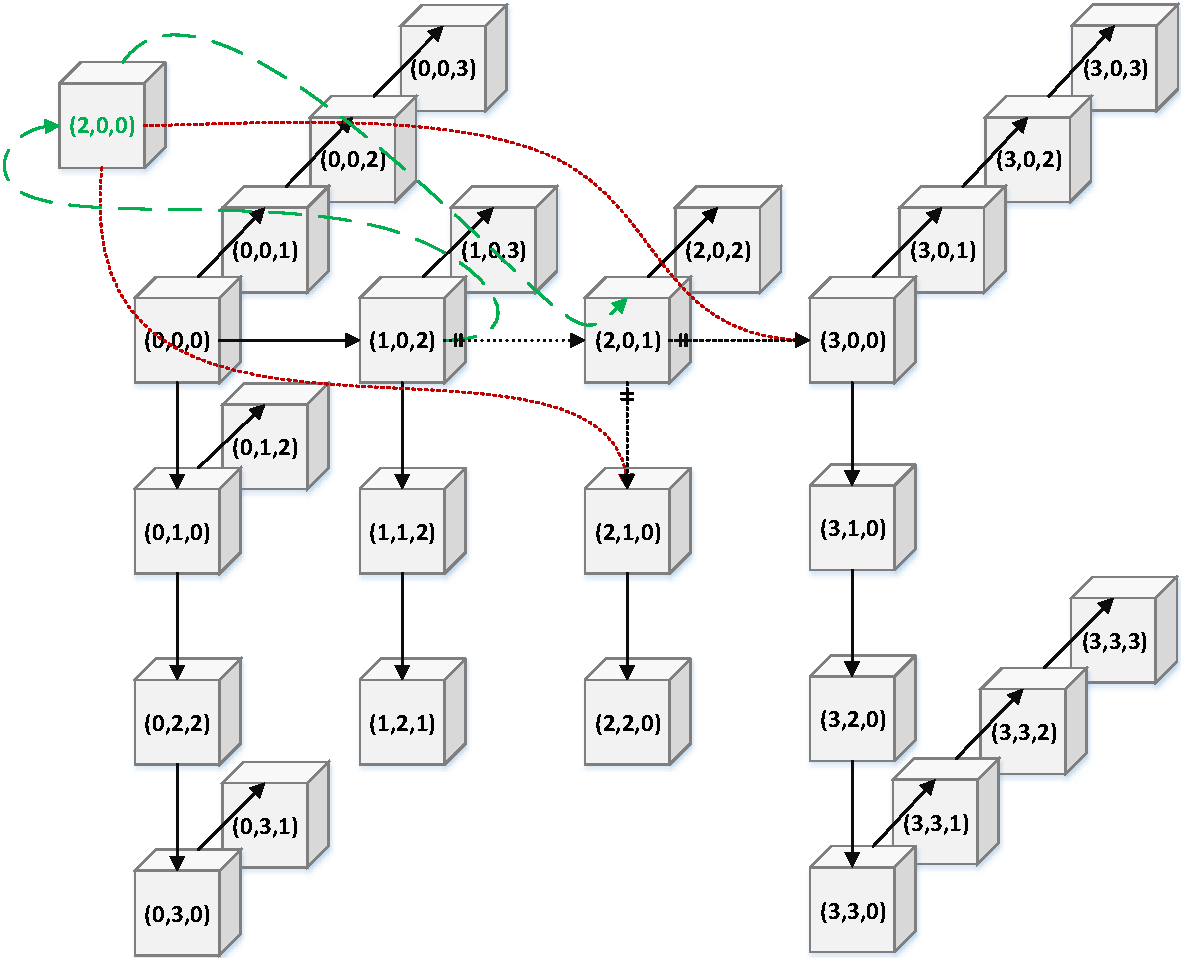
\includegraphics[width=0.95\columnwidth]{./graph/mdlist-3d-ins}
    \caption{\textsc{Insert} operation in a 3DList}
    \label{fig:mdlist3dins}
    \vspace{-0.22in}
\end{figure}

\subsection{Insertion and Deletion}
\label{sec:mdlistinsdel}
A unique property of MDList, which makes it suitable for concurrent accesses, is the locality of its insertion and deletion: each operation requires updating at most two consecutive nodes in the data structure. 
For brevity, we outline the sequential insertion and deletion in this section. 
The pseudo code is presented in Section~\ref{sec:cpqueue} when we explain in detail the concurrent versions of the algorithms.

The insertion operation involves two steps: node splicing and child adoption.
In the first step, we search and splice as depicted by the dashed green arrows in Fig.~\ref{fig:mdlist3dins}.
The appropriate insert position of the new node is determined by using a modified version of the \textsc{Search} algorithm, which keeps a record of the predecessor and the dimension of the new node (the index of the new node in its predecessor's child array).
Splicing involves pointing to the old child of the predecessor from the new node and updating the child pointer of the predecessor.
In Fig.~\ref{fig:mdlist3dins}, we insert a new node $(2,0,0)$ between its predecessor $(1,0,2)$ and the predecessor's old child $(2,0,1)$.
The new node becomes a dimension 0 child of its predecessor and the old child becomes a dimension 2 child of the new node.
The second step is needed when the dimension of the old child has been changed due to the insertion of a new node.
This extra child adoption process ensures that the nodes which are no longer accessible through the old child can be reached through the new node.
According to Definition~\ref{def:mdlist} the dimension of a node's children should be no less than the dimension of the node itself.
If the dimension of a node increases from $d$ to $d'$, its children within the range of $[d,d')$ must be adopted.
As marked by the dotted red arrows in Fig.~\ref{fig:mdlist3dins}, the new node takes over two children $(3,0,0)$ and $(2,1,0)$ from the old child $(2,0,1)$, the dimension of which increased from 0 to 2. 

The head node ($n_{head}$) of an MDList is always associated with the smallest key.
The \textsc{DeleteMin} operation should discard $n_{head}$ by identifying the node with the next smallest key ($n_{next}$), and setting it to be the new head node.
According to Section~\ref{sec:coord}, $n_{next}$ is the first non-empty child of $n_{head}$ when we reversely traverse $n_{head}$'s child array from index $D-1$ to $0$.
After becoming the new head node, $n_{next}$ has a dimensionality of $0$.
The deletion operation needs to adopt children in a similar way to that in an insertion operation: if $n_{next}$'s dimensionality decreased from $d$ to $0$, $n_{next}$ inherits $n_{head}$'s children within the range of $[0,d)$.

%\begin{figure*}[t]
    %\begin{subfigure}{0.47\textwidth}
        %\centering
        %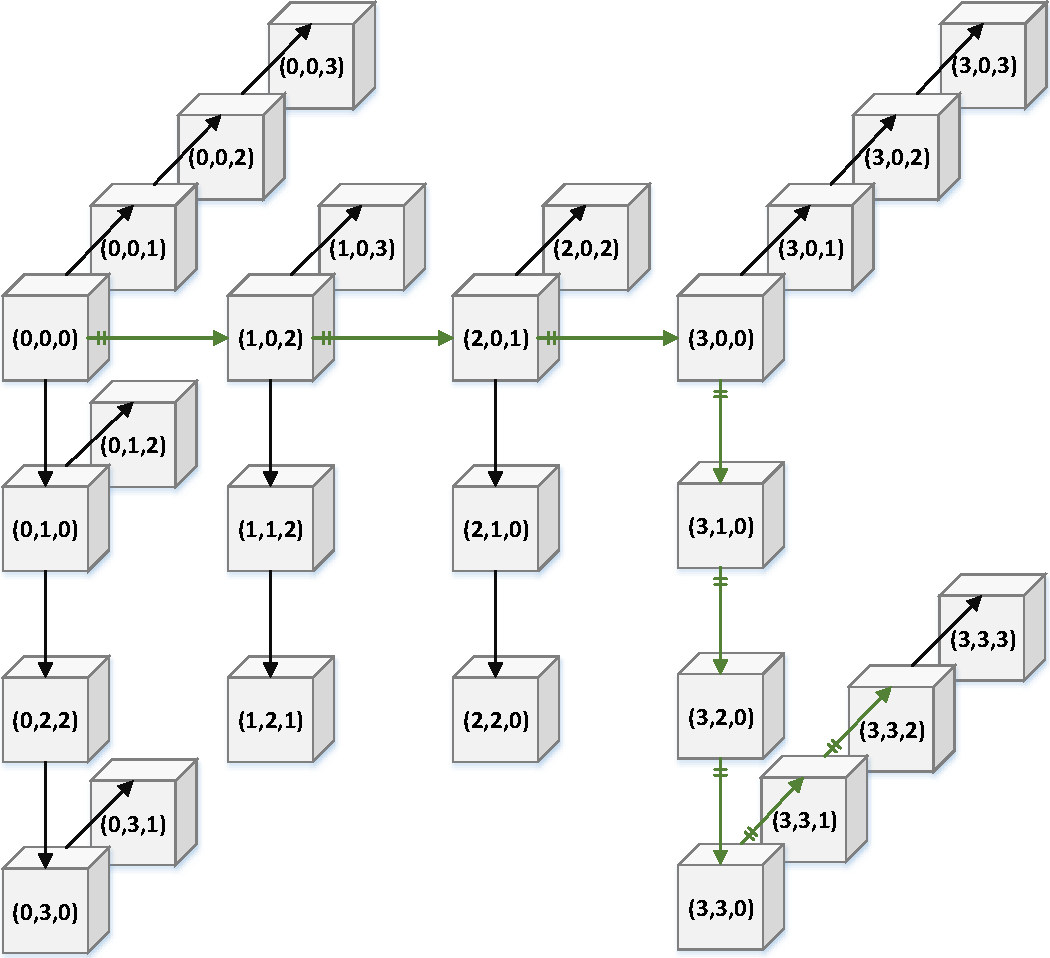
\includegraphics[width=1\columnwidth]{./graph/mdlist-3d}
        %\caption{Search for $(3,3,2)$}
        %\label{fig:mdlist3dsearch}
    %\end{subfigure}
    %\hfill
    %\begin{subfigure}{0.52\textwidth}
        %\centering
        %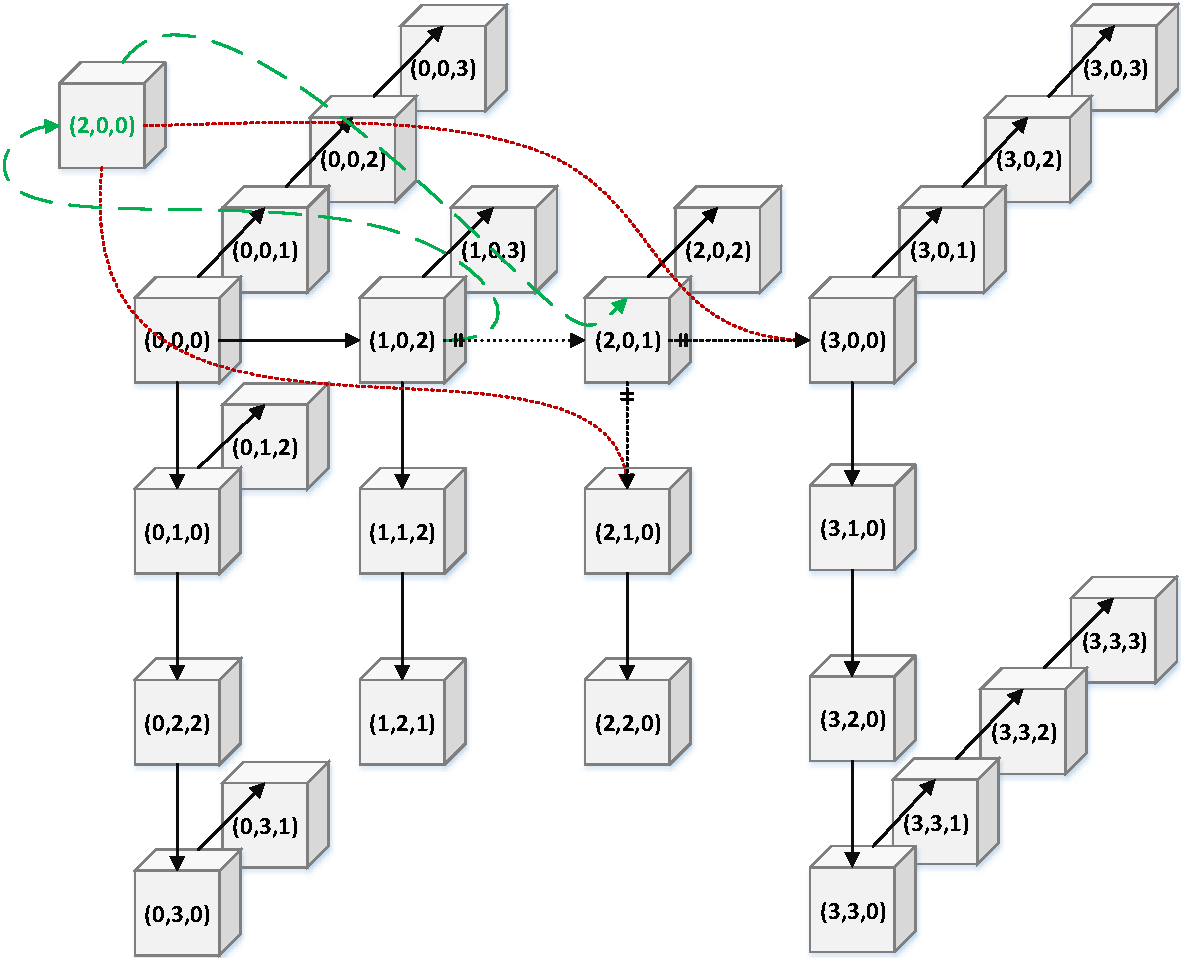
\includegraphics[width=1\columnwidth]{./graph/mdlist-3d-ins}
        %\caption{Insert New Node}
        %\label{fig:mdlist3dins}
    %\end{subfigure}
    %\caption{\textsc{Insert} operation in a 3DList}
    %\label{fig:mdlist3d}
%\end{figure*}

%\vspace{-0.05in}
\section{Lock-free Priority Queue}
\label{sec:cpqueue}
The proposed MDList provides convenient support for concurrent \textsc{Insert} operations because of its decentralized structure.
As mentioned in Section~\ref{sec:mdlistinsdel}, each insertion takes one or two steps and updates no more than two consecutive nodes.
We guarantee lock-free progress in the node splicing step by using a single-word \textsc{CompareAndSwap} (CAS) atomic synchronization primitive to atomically swing the child pointer in a similar way to that of a lock-free linked list~\cite{harris2001pragmatic}. 
To provide for lock-free progress in the child adoption step, we need to announce the operation globally using descriptor objects. 
This allows the interrupting threads to help finish the adoption in case the insertion thread is preempted.

The \textsc{DeleteMin} operation described in Section~\ref{sec:mdlistinsdel} poses a scalability challenge for concurrent executions because constant child adoption incurs heavy contention on the head node.
To avoid such performance penalties, our lock-free \textsc{DeleteMin} operations mark nodes for logical deletion~\cite{fraser2004practical}, and perform physical deletions in batch at a later stage when memory accesses are less congested.
%In addition, we use a \emph{deletion stack} that hints the logical deletion operation about the position of next smallest node. 
%This prevents deletion operations from repeatedly traversing logically deleted nodes as is observed in~\cite{linden2013skiplist,shavit2000skiplist}.
%We also design a stack rewind mechanism that allows insertions to proceed optimistically without requiring logically deleted nodes to form a prefix, as is the case in~\cite{linden2013skiplist}. 

\setlength{\columnsep}{8pt}
\begin{algorithm}[t]
    \caption{Priority Queue Structures}
    \label{alg:pqstructure}
    \vspace{-0.1in}
    \begin{multicols}{2}
        \begin{algorithmic}[1]
            \Struct{Node}
            \State \textbf{int} $key, k[D]$
            \State \textbf{void*} $val$
            \State \textbf{Node*} $child[D]$
            \State \textbf{AdoptDesc*} $adesc$
            \EndStruct
            \Statex
            \Struct{HeadNode}
            \State \textsc{\textbf{public} : Node}
            \State \textbf{int} $ver$
            \EndStruct
            \Statex
            \Struct{Stack}
            \State \textbf{Node*} $node[D]$
            \State \textbf{HeadNode*} $head$
            \EndStruct
            \Statex
            \Struct{AdoptDesc}
            \State \textbf{Node*} $curr$
            \State \textbf{int} $dp,dc$ 
            \EndStruct
            \Statex
            \Class{PriorityQueue}
            \State \textbf{const int} $D,N,R$
            \State \textbf{HeadNode*} $head$
            \State \textbf{Stack*} $stack$
            \EndClass
        \end{algorithmic}
    \end{multicols}
    \vspace{-0.1in}
\end{algorithm}

\begin{algorithm}[t]
    \caption{Pointer Marking}
    \label{alg:pointermarking}
    \begin{algorithmic}[1]
        \State \textbf{const int} $F_{adp} \gets \texttt{0x1},\;F_{prg} \gets \texttt{0x2},\;F_{del} \gets \texttt{0x1}$
        \Define{SetMark}{$p,\;m$} $(p\;|\;m)$
        \EndDefine
        \Define{ClearMark}{$p,\;m$} $(p\;\&\;\sim m)$
        \EndDefine
        \Define{IsMarked}{$p,\;m$} $(p\;\&\;m)$
        \EndDefine
    \end{algorithmic}
\end{algorithm}

\begin{figure*}[t]
    \begin{subfigure}{0.49\textwidth}
        \centering
        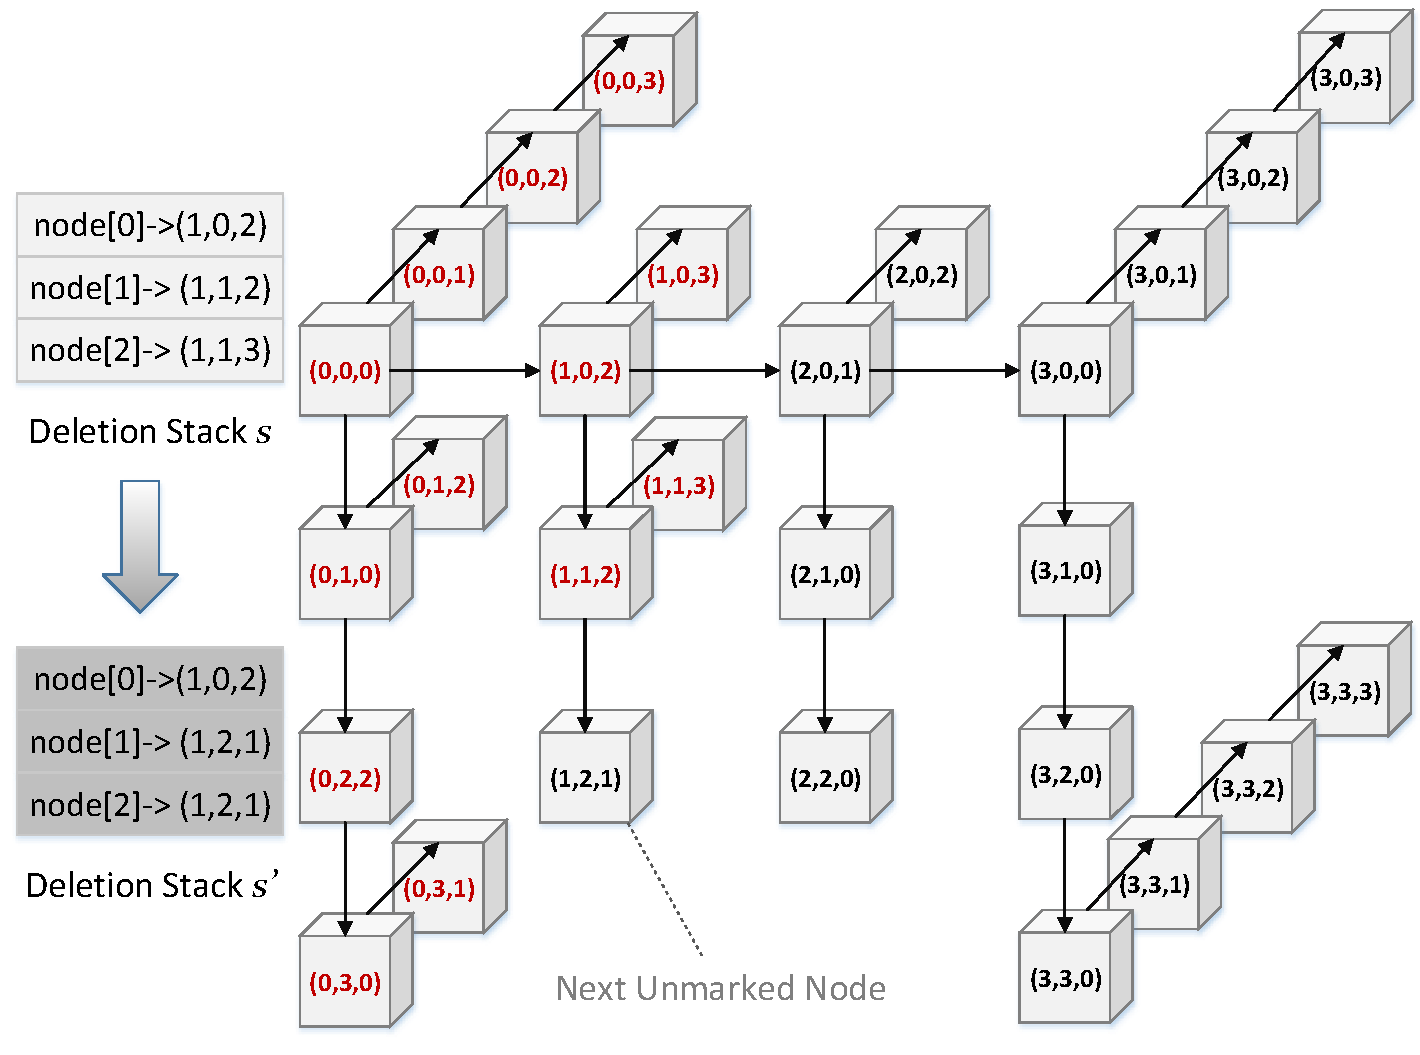
\includegraphics[width=1\columnwidth]{./graph/mdlist-3d-stack}
        \caption{Logical Deletion and Deletion Stack}
        \label{fig:mdlist3dstack}
    \end{subfigure}
    \hfill
    \begin{subfigure}{0.49\textwidth}
        \centering
        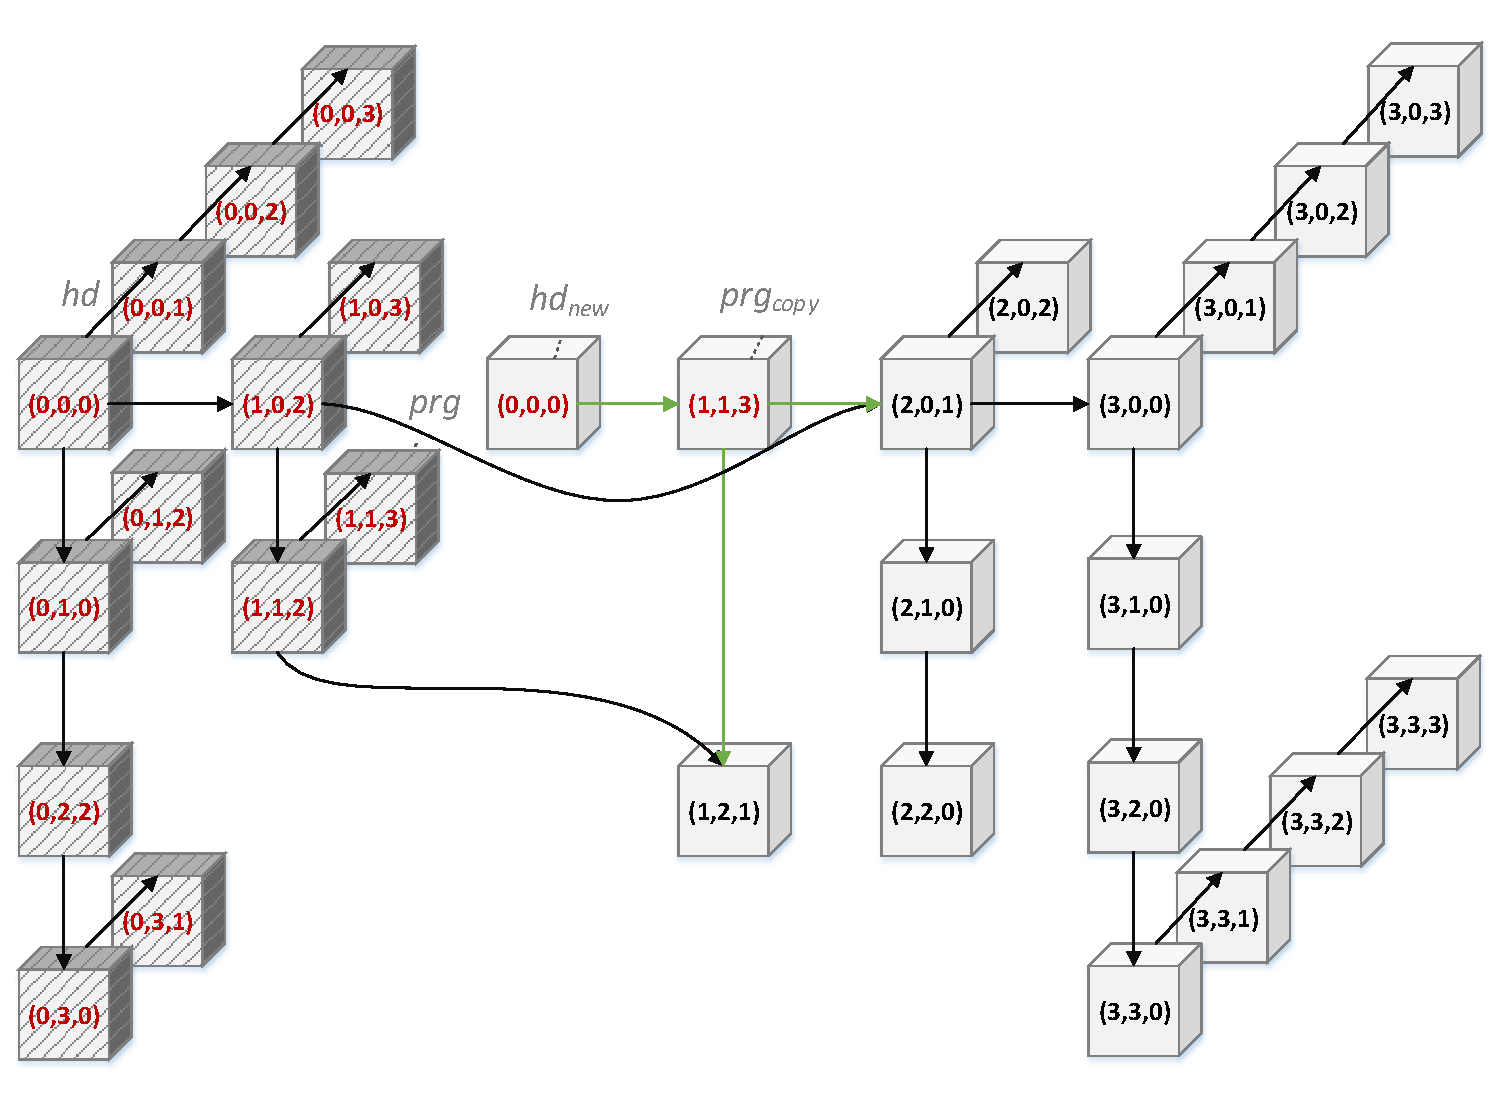
\includegraphics[width=1\columnwidth]{./graph/mdlist-3d-purge}
        \caption{Purge Node $(1,1,3)$}
        \label{fig:mdlist3dpurge}
    \end{subfigure}
    \caption{Concurrent \textsc{DeleteMin} (logically marked nodes are in red; physically removed nodes are shaded)}
    \label{fig:mdlist3ddeletemin}
    \vspace{-0.1in}
\end{figure*}

\vspace{-0.08in}
\subsection{Data Structure}
We define the structures of the lock-free priority queue in Algorithm~\ref{alg:pqstructure}. 
The descriptor object \textsc{AdoptDesc} is a data structure that stores context for a pending child adoption operation~\cite{herlihy2012art}.
The $adesc$ field in the \textsc{Node} structure signifies an interrupted child adoption task, and guides other threads to help finish it.
The \textsc{HeadNode} is a \textsc{Node} with an additional version number. 
We keep track of the version of the head node to help the insertion operation decide on a proper position for rewinding the deletion stack.
We employ the pointer marking technique described by Harris~\cite{harris2001pragmatic} to mark adopted child nodes as well as logically deleted nodes. 
The macros for pointer marking are defined in Algorithm~\ref{alg:pointermarking}.
$F_{adp}$ and $F_{prg}$ flags are co-located with the $child$ pointers while $F_{del}$ flag is co-located with the $val$ field.
A node is considered logically deleted when its $val$ field has been marked. 
%TODO: Once it is marked, we may duplex the $val$ field to hold a node pointer at a latter stage.
The \emph{deletion stack}, \textsc{Stack}, consists of an array of $D$ node pointers and a head pointer.
The pointer at index $D-1$ points to the last known logically deleted node, while pointers at indices $[0, D-1)$ point to its parents at previous dimensions.
All nodes in the stack form a path through which the next unmarked node can be reached.
The priority queue is initialized with a dummy head node, which has the minimal key 0.
The node array in the deletion stack is initially filled with the dummy head.


\vspace{-0.08in}
\subsection{Invariants}
\label{sec:inv}
We list the invariants that are satisfied by the concurrent priority queue object at all times. 
A brief proof is sketched after explaining the algorithms in details. 
By a \emph{node}, we refer to an object of type \textbf{Node} that has been allocated and successfully linked to an existing node. 
We denote the $head$ node with $ver=i$ by $head_i$, and the set of nodes that are reachable from $head_i$ by $L_i$. 
At any point of time, the set of all nodes can be denoted by $L=\bigcup_{i=0}^{m}L_i$ where $m = head.ver$.

Invariant~\ref{inv:adpflag} states that if a node has no pending child adoption task, its dimension $d$ child must have $d$ invalid child slots leaving $D-d$ valid ones.

\begin{invariant} \label{inv:adpflag}
$\forall n,n' \in L,\textsc{ClearMark}(n.child[d],F_{adp}|F_{prg}) \linebreak=n'\;\land\;n.adesc=\NIL \implies \forall i \in [0,d), \textsc{IsMarked}(n'.child$ $[i],F_{adp})=\TRUE$
\end{invariant}

\noindent Invariant~\ref{inv:reachability} states that any node in $L_i$ can be reach by following a series child pointers with non-decreasing dimensionality.
\begin{invariant} \label{inv:reachability}
    $\forall n \in L_i, \exists p=\{d_0,d_1,...,d_m\} : d_0\le d_1 \le ... \le d_m\;\land\;head_i.child[d_0].child[d_1]...child.[d_m]=n$
\end{invariant}

\noindent Invariant~\ref{inv:order} states that the ordering property described by Definition~\ref{def:mdlistsort} is kept at all times.
\begin{invariant} \label{inv:order}
    $\forall n,n' \in L, n.child[d]=n' \implies n.key < n'.key$ $\land\;\forall i \in [0, d)\; n.k[i] = n'.k[i] \land n.k[d]<n'.k[d]$
\end{invariant}

\noindent Invariant~\ref{inv:stackrelation} specify the condition for the shared $stack$ to be valid.
\vspace{-0.05in}
\begin{invariant} \label{inv:stackrelation}
    $stack.head\underbrace{.child[0]...child[0]}_{0\;or\;more\;copies}=stack.node[0]$ $\land\;\forall d \in [1,D),\;stack.node[d-1]\underbrace{.child[d]...child[d]}_{0\;or\;more\;copies}=stack.node[d]$
\end{invariant}

\subsection{Concurrent DeleteMin}
\label{sec:cpqueuedel}
One limitation with previous logical deletion approaches is that they need to traverse all logically deleted nodes before reaching the next unmarked node~\cite{linden2013skiplist,shavit2000skiplist}.
This proves to be troublesome especially for an MDList-based priority queue. 
Since an MDList is a rooted tree, reaching for the minimum node is done by a traversing procedure similar to a depth first search.
As the search extends to higher dimensions, it traverses exponentially more nodes, which slows down logical deletion.
Additionally, a naive implementation of the search algorithm based on recursion may lead to poor performance because of the overhead of function calls.  
We use a \emph{deletion stack} to hint the \textsc{DeleteMin} operation about the position of next smallest node. 
The advantage of employing the deletion stack is twofold: 1) it reduces node traversal by providing hints about the position of the next smallest node; 2) it converts the typically recursion-based search algorithm into an iteration-based one.

\subsubsection{Logical Deletion}
Fig.~\ref{fig:mdlist3dstack} illustrates an example of how the deletion stack $s$ is used in a logical deletion operation.
Nodes in red are marked for deletion.
To find the next unmarked node, the \textsc{DeleteMin} operation starts the search from the last entry of the stack instead of the head node.
It reads $s.node[2]=(1,1,3)$ and examines the dimension 2 child $s.node[2].child[2]$.
If the next smallest node exists, its earliest possible position should be $s.node[2].child[2]$.
This is because $s.node[2]$ has the largest key among known marked nodes, and its smallest children should be assigned with the highest dimensionality according to Definition~\ref{def:mdlistsort}.
In this example, node (1,1,3) does not have any child, so the operation traces back the stack to find the parent node of (1,1,3).
It reads $s.node[1]=(1,1,2)$ and examines the child $s.node[1].child[1]=(1,2,1)$, which is the next unmarked node.
After marking node (1,2,1) for deletion, the operation needs to submit an updated deletion stack $s'$ to reflect its progress. 
$s'$ is obtained by replacing the last two entries in $s$ with the newly marked node (1,2,1).

%The functionality of a deletion stack is similar to a regular LIFO stack employed by a depth-first search algorithm.
%The difference is that elements in a deletion stack can also be accessed by index, which allows for efficient stack update when the \textsc{DeleteMin} algorithm skips several logically deleted nodes. 

\begin{algorithm}[t]
    \caption{Concurrent DeleteMin}
    \label{alg:deletemin}
    \begin{algorithmic}[1]
        \Function{DeleteMin}{ }
        \State \textbf{Node*} $min \gets \NIL$
        \State \textbf{Stack*} $s_{old} \gets stack,\:s \gets \textbf{new Stack}$
        \State $*s \gets *s_{old}$ \label{l:readstack}
        \State \textbf{int} $d \gets D-1$
        \While {$d>0$} \label{l:delfor}
        \State \textbf{Node*} $last \gets s.node[d]$
        \State $\textsc{FinishInserting}(last,\;d,\;d)$
        \State \textbf{Node*} $child \gets last.child[d]$
        \State $child \gets \textsc{ClearMark}(child,F_{adp}|F_{prg})$
        \If {$child = \NIL$}
        \State $d \gets d-1$
        \State \CONTINUE
        \EndIf
        \State \textbf{void*} $val \gets child.val$
        \If {$\textsc{IsMarked}(val,\;F_{del})$} \label{l:testmark}
        \If {$\textsc{ClearMark}(val,\;F_{del}) = \NIL$} \label{l:testprg}
        \State $s.node[d:D] \gets child$ \label{l:markednode}
        \State $d \gets D-1$ \label{l:anew}
        \Else \label{l:switchhead}
        \State $s.head \gets \textsc{ClearmMark}(val,\;F_{del})$
        \State $s.node[0:D] \gets s.head,\;d \gets D-1$ \label{l:stackhead}
        \EndIf
        \ElsIf {\textsc{CAS}($\&child.val,\;val,\;\textsc{SetMark}(val,F_{del}))$} \label{l:delcas}
        \State $s.node[d:D] \gets child,\;min \gets child$ \label{l:delstackupdate}
        \State $\textsc{CAS}(\&stack,\;s_{old},\;s)$ \label{l:stackupdate}
        \If {$marked\_node > R \AND not\_purging$} \label{l:checkpurge}
        \State \Call{Purge}{$s.head,\;s.node[D-1]$}
        \EndIf
        \State \BREAK
        \EndIf
        \EndWhile
        \State \Return $min$
        \EndFunction
    \end{algorithmic}
\end{algorithm}

Algorithm~\ref{alg:deletemin} lists the concurrent \textsc{DeleteMin} operation for a $D$-dimensional list.
The operation backtracks the stack $s$ until it reaches the top (line~\algref{alg:deletemin}{l:delfor}) or finds an entry $s.node[d]$ whose child $s.node[d].child[d]$ is not marked (line~\algref{alg:deletemin}{l:delcas}).
In concurrent executions, $s.node[d].child[d]$ might have been marked by competing \textsc{DeleteMin} threads.
If this is the case, as detected by the condition check on line~\algref{alg:deletemin}{l:testmark}, the operation updates the local copy of the deletion stack (line~\algref{alg:deletemin}{l:markednode})\footnote{We use indexing notion $[a:b]$ to address elements within the range of $[a, b)$.} and starts anew (line~\algref{alg:deletemin}{l:anew}).
Note that the operation does not need to examine $s.node[d].child[d'],\;\forall d' \in [d+1,D)$ because it must have examined them in previous iterations given that $s$ is valid (Invariant~\ref{inv:stackrelation}).
After successfully marking a node, the operation updates the shared stack (line~\algref{alg:deletemin}{l:stackupdate}) using CAS.

\begin{algorithm}[ht]
    \caption{Batch Physically Deletion}
    \label{alg:purge}
    \begin{algorithmic}[1]
        \Function{Purge}{$\textbf{HeadNode*}\;hd,\;\textbf{Node*}\;prg$}
        \If {$hd \neq head$} \Return
        \EndIf
        \State \textbf{Node*} $hd_{new} \gets \textbf{new Node},\;prg_{copy} \gets \textbf{new Node}$ 
        \State $*prg_{copy} \gets *prg,\;prg_{copy}.child[0:D] \gets \NIL$
        \State $hd_{new}.val \gets F_{del},\;hd_{new}.ver \gets hd.ver+1$ \label{l:seqinc}
        \For {$d \gets 0,\;pvt \gets hd;\;d < D$} \label{l:prgfor}
        \If{!\Call{LocatePivot}{ }} \label{l:prgcheckrestart}
        \State $pvt \gets hd,\;d \gets 0$ \label{l:prgrestart}
        \State \CONTINUE
        \EndIf
        \If {$pvt = hd$}
        \State $hd_{new}.child[d] \gets child$ \label{l:hdchild}
        \State $prg_{copy}.child[d] \gets F_{del}$
        \Else
        \State $prg_{copy}.child[d] \gets child$ \label{l:prgchild}
        \If {$d = 0 \OR prg_{copy}.child[d-1] = F_{del}$}
        \State $hd_{new}.child[d] \gets prg_{copy}$ 
        \EndIf
        \EndIf
        \State $d \gets d+1$
        \EndFor
        \State $hd.val \gets \textsc{SetMark}(prg,F_{del}))$ \label{l:markprg}
        \State $prg.val \gets \textsc{SetMark}(hd_{new},F_{del}))$ \label{l:markhdnew}
        \State $head \gets hd_{new}$
        \EndFunction
        \Statex
        \Inline{LocatePivot}{ }
        \While{$prg.k[d] > pvt.k[d]$} \label{l:findprg}
        \State $\textsc{FinishInserting}(pvt,\;d,\;d)$ 
        \State $pvt \gets \textsc{ClearMark}(pvt.child[d], F_{adp}|F_{prg})$
        \EndWhile
        \Repeat
        \State $child \gets pvt.child[d]$ \label{l:pvtchild}
        \Until {$\textsc{CAS}(\&pvt.child[d],child,\textsc{SetMark}(child,F_{prg})$ $ \indent\OR \textsc{IsMarked}(child,\;F_{adp} | F_{prg})$} \label{l:prgwhile}
        \EndInline
        \If {$\textsc{IsMarked}(child, F_{prg})$ \label{l:prgcheckrestart}}
        \State $child \gets \textsc{ClearMark}(child, F_{prg})$
        \State \Return \TRUE
        \Else ~\Return \FALSE
        \EndIf
    \end{algorithmic}
\end{algorithm}

\subsubsection{Physical Deletion}
The physical deletion operation, or \textsc{Purge}, discards logically deleted nodes in batch and prepare them for memory reclamation.
The existence of purge is not needed for correct execution of our priority queue algorithm, but timely purges ensure efficient execution of the logical deletion operations.
We initiate a physical deletion if the logical deletion operation had to traverse too many marked nodes before reaching the unmarked node (line~\algref{alg:deletemin}{l:checkpurge}).
The threshold $R$ should be sufficient large such that the purge takes advantage of batch processing, but not too large to hinder the progress of logical deletion operations. 
We give more details on choosing appropriate threshold $R$ in Section~\ref{sec:experiment}.

In Fig.~\ref{fig:mdlist3dpurge}, we purge the group of logically deleted nodes by introducing a new dummy head node ($hd_{new}$).
The layout of both the purged nodes (shaded ones) and the remaining nodes (black ones), as well as the linkage between the two groups, are preserved.
This effectively produces two valid MDLists rooted at $hd$ and $hd_{new}$ respectively.
Subsequent insertion operations will start from $hd_{new}$, but ongoing insertions that started from $hd$ can still finish.
The placeholder node $prg_{copy}$, which is a copy of $prg$, is necessary to maintain the dimensionality of the remaining nodes.
Without $prg_{copy}$, node (1,2,1) has to be promoted as the dimension 0 child of $hd_{new}$ in the new MDList.
This alternation to the layout of the remaining nodes causes inconsistent dimensionality, e.g., node (1,2,1) is still the dimension 1 child of node (1,1,2) when accessed through the old MDList head $hd$.

Algorithm~\ref{alg:purge} lists the detailed purge operation.
Given the last node to purge ($prg$), the \textsc{LocatePivot} function\footnote{For clarity of presentation, we use the notion of \textbf{inline} functions, which have implicit access to caller's local variables without explicit argument passing.} identifies for each dimension $d\in[0,D)$ a pivot node ($pvt$) such that $\forall i \in [0,d),\;pvt.k[i]=prg.k[i] \land pvt.k[d] \le prg.k[d]$. 
The pivot node ($pvt$) divides the $d$-dimensional sublist such that itself along with its predecessors will be purged while its successors will be kept.
$pvt.child[d]$ is linked to either $hd_{new}$ or $prg_{copy}$ in a manner that preserves its current dimensionality.
To prevent $pvt.child[d]$ from being changed by concurrent insertions, we employ the same pointer marking technique as the child adoption process using a different flag $F_{prg}$ (line~\algref{alg:purge}{l:prgwhile}).

After the purge, nodes between $hd$ and $prg$ can be safely reclaimed when all threads have concluded their operations on the old MDList rooted at $hd$.
We use an epoch-based garbage collector~\cite{pugh1990concurrent,fraser2004practical} to reclaim the memory of dynamically allocated nodes.
This kind of garbage collection is light weight and efficient, but it requires that the objects which are longer reference to be explicitly added to a garbage list.
Since we only process the physical deletion in the purge function, the thread performing purge are solely responsible for putting purged nodes on the list. 
Each purge creates a garbage list identified by the version of the head being purged.
Every time a thread starts an operation it observes the current head version: for \textsc{Insert} it is $head.ver$; for \textsc{DeleteMin} it is $stack.head.ver$.
Once all threads have observed the same head version $v$, the garbage list associated with $v-1$ can be safely reclaimed.
For the descriptor objects and deletion stacks, we employ reference courting~\cite{michael1995correction} because those are transient objects that do not reference each other.
We could reuse them as quickly as possible so that the heap need not to accommodate defunct-but-unusable descriptors and stacks.


\subsubsection{Preservation of Invariants}
\noindent \textsc{DeleteMin} preserves Invariant~\ref{inv:adpflag}.
\begin{proof}
    Both logical deletion and physical deletion operations do not modify nodes' $F_{adp}$ flags.
\end{proof}

\noindent\textsc{DeleteMin} preserves Invariant~\ref{inv:reachability}.
\begin{proof}
    Logical deletion does not alter linkage among nodes.
    Physical does not alter existing links, so invariant holds for $n \in L_i,\;where\;i=hd.ver$.
    It introduces new links that keep the invariant for $n \in L_{i+1},\;where\;i+1=hd_{new}.ver$ because $\forall d \in [0,D),\;pvt.child[d] =hd_{new}.child[d] \lor pvt.child[d]=prg_{copy}.child[d]$
\end{proof}

\noindent\textsc{DeleteMin} preserves Invariant~\ref{inv:order}.
\begin{proof}
    Logical deletion does not alter linkage among nodes.
    Physical deletion preserves the ordering property because of the condition check on line~\algref{alg:purge}{l:findprg}.
\end{proof}

\noindent\textsc{DeleteMin} preserves Invariant~\ref{inv:stackrelation}.
\begin{proof}
    The invariant trivially holds on line~\algref{alg:deletemin}{l:stackhead}.
    On lines~\algref{alg:deletemin}{l:delstackupdate} and~\algref{alg:deletemin}{l:markednode}, The algorithm sets $s.node[d:D]$ to $child$.
    The invariant holds because $child = s.node[d].child[d]$.
\end{proof}

\begin{algorithm}[t]
    \caption{Concurrent Insert}
    \label{alg:insert}
    \begin{algorithmic}[1]
        \Function{Insert}{$\textbf{int}\;key,\;\textbf{void*}\;val$}
        \State $\textbf{Stack*}\; s \gets \textbf{new Stack}$
        \State $\textbf{Node*}\; node \gets \text{\textbf{new Node}}$
        \State $node.key \gets key,\;node.val \gets val$
        \State $node.k[0:D] \gets \text{\textsc{KeyToCoord}}(key)[0:D]$
        \State $node.child[0:D] \gets \NIL$
        \While{\TRUE}
        \State $\textbf{Node*}\; pred \gets \NIL,\;curr \gets head$\label{l:insfromhead}
        \State $dp \gets 0,\;dc \gets 0$ 
        \State $s.head \gets curr$ \label{l:recordhead}
        \State \Call{LocatePred}{ } \label{l:locpre1}
        \If{$dc=D$} \label{l:dupnode}
        %TODO: cannot quit yet, check deletion and re-enable node if needed. We can keep it like this if input keys are unique
        \State \BREAK
        \EndIf
        \State \Call{FinishInserting}{$curr,\;dp,\;dc$} \label{l:endhelp}
        \State \Call{FillNewNode}{ } \label{l:callfillnode}
        \If {$\text{\textsc{CAS}}(\&pred.child[dp],\;curr,\;node)$} \label{l:link}
        \State \Call{FinishInserting}{$node,\;dp,\;dc$} \label{l:adoptself}
        \State \Call{RewindStack}{ } \label{l:rewind}
        \State \BREAK
        \EndIf
        \EndWhile
        \EndFunction
        \Statex
        \Inline{LocatePred}{ } \label{l:locpre2}
        \While {$dc < D$}
        \While {$curr\neq\NIL \AND node.k[dc] > curr.k[dc]$} \label{l:predcheck1}
        \State $pred \gets curr,\:dp \gets dc$ \label{l:dp}
        \State \Call{FinishInserting}{$curr,\;dc,\;dc$} \label{l:help}
        \State $curr \gets curr.child[dc]$ \label{l:dcchild}
        \EndWhile
        \If {$curr=\NIL \OR node.k[dc] < curr.k[dc]$} \label{l:predcheck2}
        \State \BREAK
        \Else
        \State $s.node[dc] \gets curr,\;dc \gets dc+1$ \label{l:dc}
        \EndIf
        \EndWhile
        \EndInline
        \Statex
        \Inline{FillNewNode}{ } \label{l:fillnode}
        \State $node.adesc \gets \NIL$  \label{l:beginfill}
        \If {$dp < dc$} \label{l:filldesc}
        \State $node.adesc \gets \text{\textbf{new AdoptDesc}}$
        \State $node.adesc.curr \gets curr$ 
        \State $node.adesc.dp \gets dp,\;node.adesc.dc \gets dc$ 
        \EndIf
        \State $node.child[0:dp] \gets F_{adp}$ \label{l:initadp}
        \State $node.child[dp:D] \gets \NIL$ 
        \State $node.child[dc] \gets curr$ \label{l:endfill}
        \EndInline
    \end{algorithmic}
\end{algorithm}

\begin{algorithm}[t]
    \caption{Child Adoption}
    \label{alg:adoption}
    \begin{algorithmic}[1]
        \Function{FinishInserting}{$\textbf{Node*}\:n,\;\textbf{int}\:dp,\;\textbf{int}\;dc$}
        \If {$n = \NIL$}
        \State \Return
        \EndIf
        \State \textbf{AdoptDesc*} $ad \gets n.adesc$
        \If {$ad=\NIL \OR dc < ad.dp \OR dp > ad.dc$}
        \State \Return
        \EndIf
        \State \textbf{Node*} $child,\;curr \gets ad.curr$ 
        \State \textbf{int} $dp \gets ad.dp,\;dc \gets ad.dc$
        \For {$i \in [dp, dc)$} \label{l:adoptionfor}
        \State $child \gets \textsc{FetchAndOr}(\&curr.child[i],\;F_{adp})$ \label{l:setadp} 
        \State $child \gets \textsc{ClearMark}(child,\;F_{adp})$
        \State $\text{\textsc{CAS}}(\&n.child[i],\;\NIL,\;child)$ \label{l:adopt}
        \EndFor
        \State $n.adesc \gets \NIL$
        \EndFunction
    \end{algorithmic}
\end{algorithm}



\subsection{Concurrent Insert}
\label{sec:cpqueueins}
Algorithm~\ref{alg:insert} lists the concurrent \textsc{Insert} function.
\textsc{LocatePred}, which is an extension of the sequential search function (Algorithm~\ref{alg:search}), determines the target position by locating the new node's immediate parent $pred$ and child $curr$ (line~\algref{alg:insert}{l:locpre1} and~\algref{alg:insert}{l:locpre2}).
We link $pred.child[dp]$ to the new node on line~\algref{alg:insert}{l:link}.
The new node should be inserted as the dimension $dp$ child of the $pred$ node, while a non-empty $curr$ node will become the dimension $dc$ child of the new node.
Regardless of the dimensionality of the data structure, $pred$ and $curr$ are the only nodes that is updated by an insertion.
The CAS-based loop restarts when the CAS fails under three circumstances: 1) the desired child slot has been updated by a competing insertion; 2) the desired child slot has been marked invalid by a child adoption process; and 3) the desired child slot has been marked invalid by a purge operation.
The deletion stack needs to be rewound (line~\algref{alg:insert}{l:rewind}) if the new node was inserted into a position that cannot be reached by subsequent \textsc{DeleteMin} operations.
We explain this synchronization mechanism in details in Section~\ref{sec:cpqueuerewind}.

%The conditional check on line~\algref{alg:insert}{l:dupnode} is true when a node with the same coordinates already exists, thus the insertion terminates.
%The pointers within the range $[0, dp)$ of the new node's child array are marked with $F_{adp}$.
%This effectively invalidates these positions for future insertions.
%The pointers within the range $[dp, D]$ are set to \textsc{NIL} meaning they are available for attaching child nodes.

\subsubsection{Helping with Child Adoption}
The \textsc{FinishiInserting} function in Algorithm~\ref{alg:adoption} performs child adoption on a given node $n$.
Child adoption is necessary when the insertion of $n$ demotes its immediate child node ($curr$) to a higher dimension (line~\algref{alg:insert}{l:filldesc}).
As described in Section~\ref{sec:mdlistinsdel}, $n$ needs to adopt multiple children $curr.child[i],\;i\in [dp,dc)$.
Before a child pointer can be copied, we must safeguard it so that it cannot be changed by concurrent insertions while the copy is in progress.
This is done by setting the $F_{adp}$ flag in the child pointers (line~\algref{alg:adoption}{l:setadp}).
Once the flag is set either by this thread or by other threads, the function proceeds to copy the pointer to $n$ (line~\algref{alg:adoption}{l:adopt}). 
Finally, the descriptor field in $n$ is cleared to designate the operation's completion.

The child adoption task is usually completed by the thread that just successfully inserted node $n$ (line~\algref{alg:insert}{l:adoptself}).
However, helping is enforced if another thread tries to read $n.child[d],\;d \in[n.adesc.dp,n.adesc.dc)$ before the insertion thread could finish the child adoption task.
For example, on line~\algref{alg:insert}{l:help} \textsc{LocatePred} helps $curr$ node prior to reading $curr.child[dc]$.
The search process can continue without restart because the child adoption appears transparent to traversing operations, i.e., the helping task does not alter already traversed nodes.
In our algorithms, all accesses to a node's child pointers are lead by a call to \textsc{FinishInserting}, which enforces child adoption and ensures consistency.

\begin{algorithm}[t]
    \caption{Rewind Deletion Stack}
    \label{alg:rewind}
    \begin{algorithmic}[1]
        \Inline{RewindStack}{}
        \State $\textbf{Stack*}\;s_{old} \gets stack$
        \Repeat
        \If{$s.head.ver = s_{old}.head.ver$} \label{l:samehead}
        \If{$node.key \le s_{new}.node[D-1].key$}
        \State $s.node[dp:D] \gets pred$ \label{l:rewindpred}
        \ElsIf {$first\;iteration$} $*s \gets *s_{new}$ \label{l:asitwas}
        \Else ~\BREAK \label{l:norewind1}
        \EndIf
        \ElsIf {$s.head.ver > s_{old}.head.ver$} \label{l:newerhead}
        \State \textbf{Node*} $prg \gets \textsc{ClearMark}(s_{old}.head.val)$
        \If {$prg.key \le s_{old}.node[D-1].key$}
        \State $s.head \gets \textsc{ClearMark}(prg.val, F_{del})$ \label{l:rewindnewhead}
        \State $s.node[0:D] \gets s.head$ \label{l:gethead1}
        \ElsIf {$first\;iteration$} $*s \gets *s_{old}$
        \Else ~\BREAK \label{l:norewind2}
        \EndIf
        \Else
        \State \textbf{Node*} $prg \gets \textsc{ClearMark}(s.head.val)$
        \If {$prg.key \le node.key$}
        \State $s.head \gets \textsc{ClearMark}(prg.val,\; F_{del})$
        \State $s.node[0:D] \gets s.head$ \label{l:gethead2}
        \Else ~$s.node[dp:D] \gets pred$ \label{l:getpred2}
        \EndIf
        \EndIf
        \Until {$\textsc{CAS}(\&stack,\;s_{new},\;s) \OR \textsc{IsMarked}(node.prg,$ $F_{del})$} \label{l:rewindcas}
        \EndInline
    \end{algorithmic}
\end{algorithm}

\begin{figure*}[t]
    \begin{subfigure}{0.33\textwidth}
        \centering
        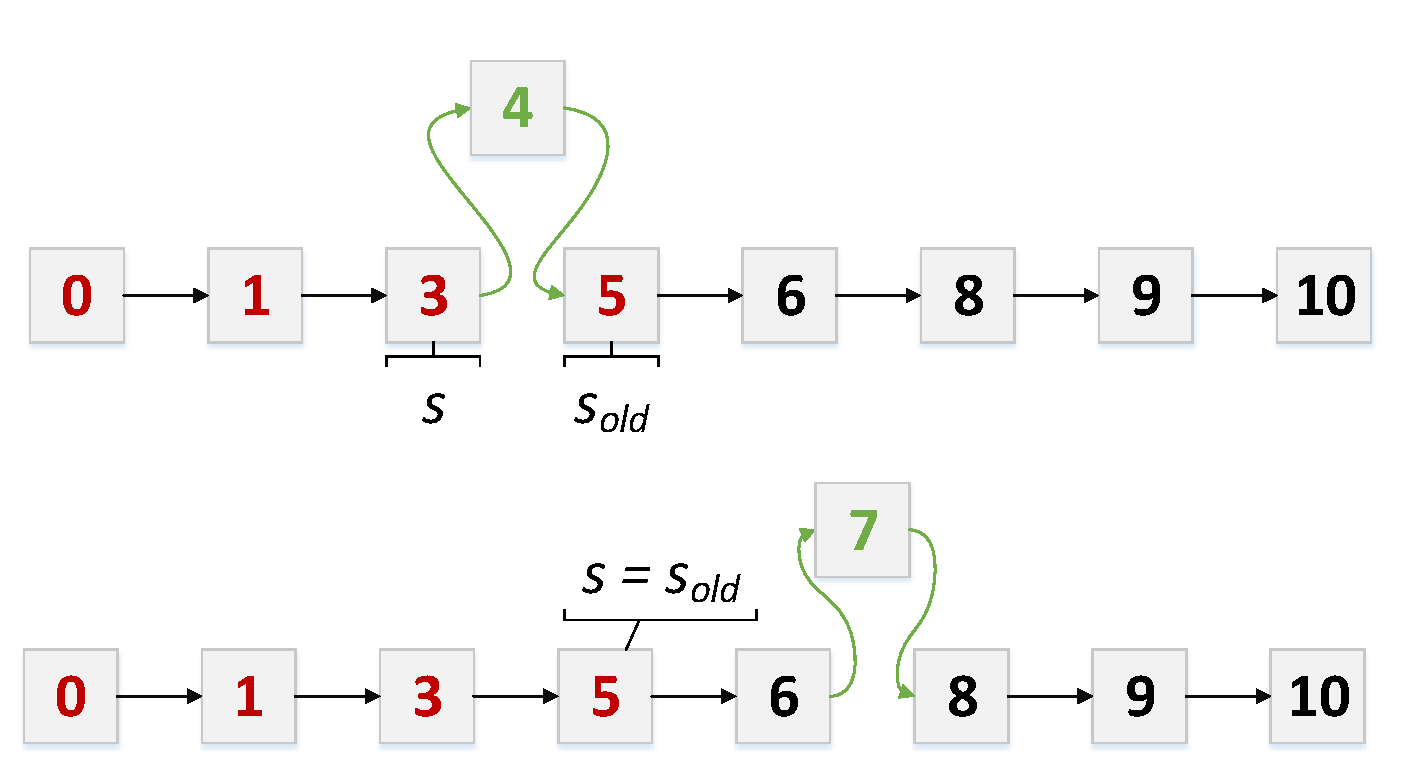
\includegraphics[width=1\columnwidth]{./graph/mdlist-3d-rewind1.pdf}
        \caption{$s.head.ver = s_{old}.head.ver$}
        \label{fig:rewind1}
    \end{subfigure}
    \hfill
    \begin{subfigure}{0.33\textwidth}
        \centering
        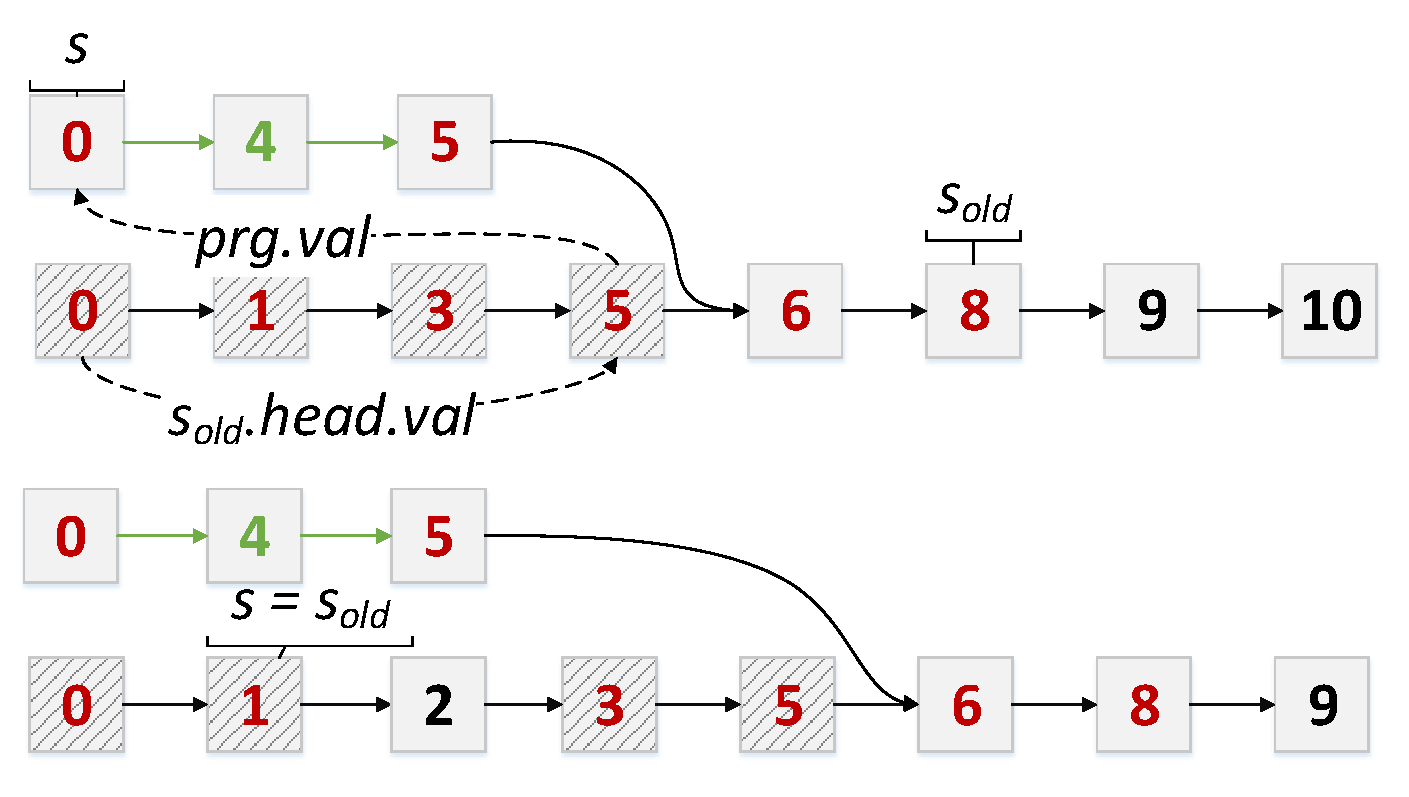
\includegraphics[width=1\columnwidth]{./graph/mdlist-3d-rewind2.pdf}
        \caption{$s.head.ver > s_{old}.head.ver$}
        \label{fig:rewind2}
    \end{subfigure}
    \hfill
    \begin{subfigure}{0.33\textwidth}
        \centering
        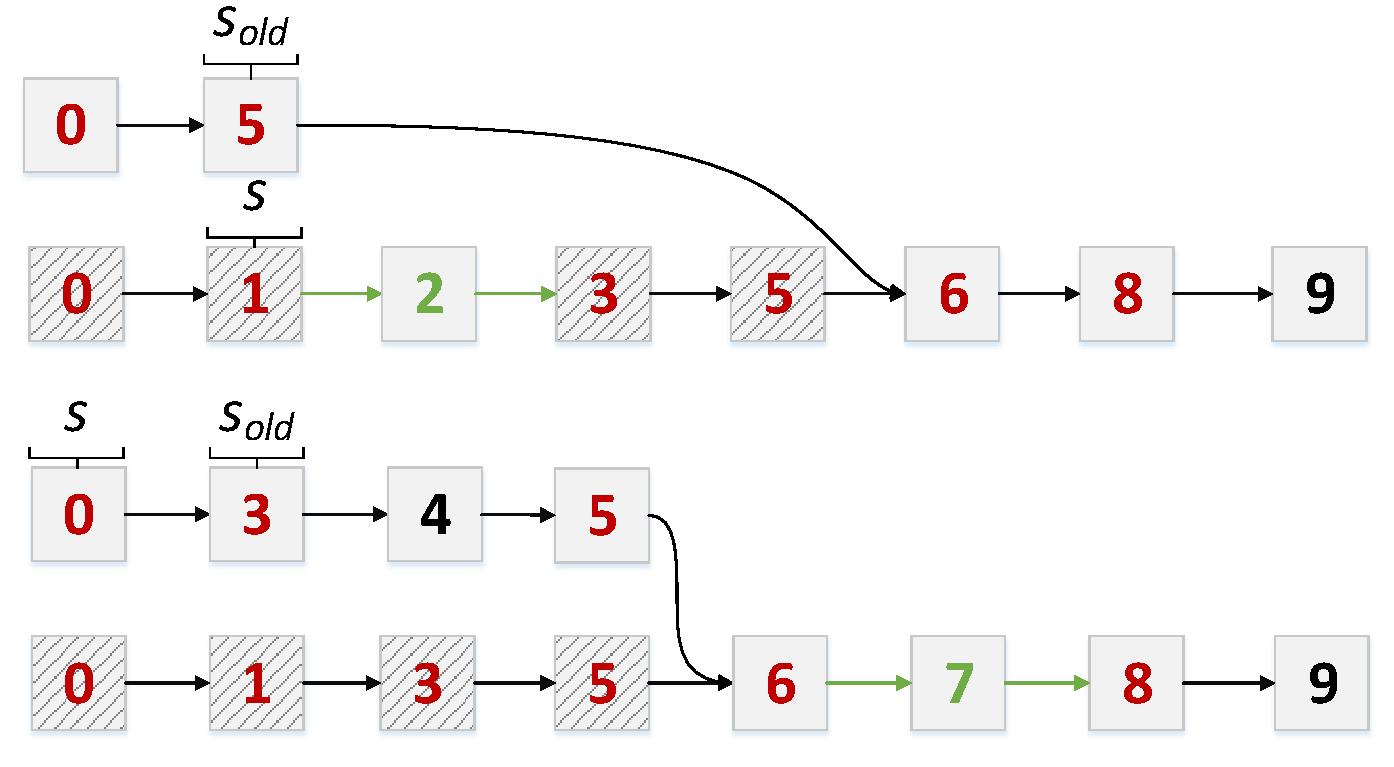
\includegraphics[width=1\columnwidth]{./graph/mdlist-3d-rewind3.pdf}
        \caption{$s.head.ver < s_{old}.head.ver$}
        \label{fig:rewind3}
    \end{subfigure}
    \caption{Three stack rewind scenarios (black nodes are normal; red nodes are logically deleted; shaded nodes are purged)}
    \label{fig:rewind}
    \vspace{-0.15in}
\end{figure*}
 
\subsubsection{Synchronizing Insert with DeleteMin}
\label{sec:cpqueuerewind}
In our design, \textsc{Insert} and \textsc{DeleteMin} are synchronized through the stack rewind mechanism.
Intuitively, a deletion thread ``advances'' the deletion stack while an insertion thread ``rewinds'' the stack when it detects that the stack points to a position beyond the new node. 
The insertion rewinds the stack to a position before the newly inserted node so that it is made visible to future deletion threads. 
In contrast with the previous approach~\cite{linden2013skiplist}, in which logically deleted nodes are required to form a prefix, our approach allows insertion threads to proceed optimistically without blocking deletion threads until the new nodes are in place. 

Algorithm~\ref{alg:rewind} determines the exact position of rewound stack $s$ based on the temporal relation between $s$ and $s_{old}$ (as ordered by head version $head.ver$), and categorizes the rewinds into three scenarios as shown in Fig.~\ref{fig:rewind}.
For simplicity, we depict logical ordering of nodes rather than the physical layout of the MDList.
Fig.~\ref{fig:rewind1} illustrate the first case, in which the head node is unchanged (line~\algref{alg:rewind}{l:samehead}).
If $s_{old}$ points to a node with larger key than that of the new node, we rewind the stack to the new node's predecessor (line~\algref{alg:rewind}{l:rewindpred}).
Otherwise, deletion threads have yet to reach the new node and we can skip the rewind except for the first iteration, in which case we update the stack as it is to make sure the new node will not be skipped by concurrent deletions (line~\algref{alg:rewind}{l:asitwas}).

In the second case, $s$ is more recent than $s_{old}$, which means $s_{old}.head$ has been purged.
As shown in the top diagram of Fig.~\ref{fig:rewind2}, we need to rewind the stack to the new head given by $prg.val$ to ensure the new node is reachable (line~\algref{alg:rewind}{l:rewindnewhead}).
During a purge operation, we duplex nodes' $val$ fields to store two convenient pointers (dashed arrows in Fig.~\ref{fig:rewind2}): one in the purged head node pointing to the last purged node (line~\algref{alg:purge}{l:markprg}); another in the last purged node pointing to the new head node(line~\algref{alg:purge}{l:markhdnew}).
The \textsc{DeleteMin} operation will switch to the new head if it detects the node has been purged (line~\algref{alg:deletemin}{l:switchhead}).
We thus keep the stack as it is if $s_{old}$ has not reached the last purged node. 
This is depicted in the bottom diagram of Fig.~\ref{fig:rewind2}.

In the last case, $s_{old}$ is more recent (line~\algref{alg:rewind}{l:newerhead}).
If the new node is inserted before the last purged node, as shown in the top diagram of Fig.~\ref{fig:rewind3}, it cannot be reached through $s_{old}$.
We rewind the stack to the predecessor.
On the other hand, if the new node is inserted after the last purged node (bottom of Fig.~\ref{fig:rewind}), we rewind the stack to the next head ($prg.val$) regardless the position of the $s_{old}$ to ensure reachability .

\subsubsection{Preservation of Invariants}
\textsc{Insert} preserves Invariant~\ref{inv:adpflag}.
\begin{proof}
    By observing the statements at line~\algref{alg:insert}{l:initadp} and~\algref{alg:adoption}{l:setadp} we see that the $F_{adp}$ flags are properly initialized before linking a new node to its predecessor and updated properly whenever a child is adopted.
\end{proof}

\noindent\textsc{Insert} preserves Invariant~\ref{inv:reachability}.
\begin{proof}
    At the start, the structure contains a single dummy $head$ node and the invariant holds trivially. 
    Any new node is initially placed at a position reachable from $head$ because the node traversed by \textsc{LocatePred} form a consecutive path $p'$.
    Note the condition checks in (line~\algref{alg:insert}{l:predcheck1} and~\algref{alg:insert}{l:predcheck2}), we have $i<j \implies d_i \leq d_j \;\forall d_i,d_j \in p'$.
    Though the path may be altered by subsequent insertions, we do not unlink nodes from the data structure.
    The claim follows by noting that an insertion either adds a new node to $p'$ or replaces an existing node in $p'$, i.e.,$p'\subseteq p$. 
\end{proof}

\noindent\textsc{Insert} preserves Invariant~\ref{inv:order}.
\begin{proof}
    Initially the invariants trivially holds.
    The linkage among nodes can be changed by insertion, child adoption.
    Insert preserves the invariants because the condition checks on line~\algref{alg:insert}{l:predcheck1} and~\algref{alg:insert}{l:predcheck2} guarantee that $\forall i \in [0, dp)\; pred.k[i] = node.k[i] \land pred.k[dp]<node.k[dp]$.
    Child adoption preserves the invariant because $\forall i \in [dp, dc)\; node.k[i] = curr.k[i] < curr.child[i].k[i]$.
\end{proof}

\noindent \textsc{Insert} preserves Invariant~\ref{inv:stackrelation}.
\begin{proof}
    The invariant holds trivially on line~\algref{alg:rewind}{l:gethead1} and~\algref{alg:rewind}{l:gethead2}.
    The updates on line~\algref{alg:rewind}{l:rewindpred} and~\algref{alg:rewind}{l:getpred2} keep the stack entries within the range of $(dp:D)$ valid by assigning them the same value $pred$. 
    The entries within the range of $[0,dp]$ are valid because \textsc{LocatePred} updates them by following a path starting from $s.head$ (line~\algref{alg:insert}{l:recordhead}) such that $\forall dc\in[1,dp],\;s.node[dc]=s.node[dc-1]\underbrace{.child[dc]...child[dc]}_{0\;or\;more\;copies}$ (line~\algref{alg:insert}{l:dcchild} and~\algref{alg:insert}{l:dc}).
\end{proof}

\section{Correctness}
\label{sec:correctness}
In this section, we sketch a proof of the main correctness property of the presented priority queue algorithm, which is quiescent consistency. 
Additionally, we discuss how stricter correctness conditions such as linearizability can be guaranteed through the use of time-stamps.
We explain the relaxation of the \textsc{DeleteMin} operation when the concurrent object is executed without quiescent periods. 
We begin by defining the \emph{abstract state} of a sequential priority queue and then show how to map the internal state of our concrete priority queue object to the abstract state.
We denote the abstract state of a sequential priority queue to be a set $P$.
Equation~\ref{eq:insert} specifies that an \textsc{Insert} operation grows the set if the key being inserted does not exist.
Equation~\ref{eq:delete1} and~\ref{eq:delete2} specify that a \textsc{DeleteMin} operation shrinks a non-empty set by removing the key-value pair with the smallest key.

\begin{equation} \label{eq:insert}
    \textsc{Insert}(\langle k,v \rangle)= \begin{cases}
        P \cup \{\langle k,v\rangle\} & \forall \langle k',v'\rangle \in P\;,\;k' \neq k\\
        P & \exists \langle k',v' \rangle \in P : k'=k
    \end{cases}
\end{equation}

\begin{gather}
    \label{eq:delete1}
    \textsc{DeleteMin}()= \begin{cases}
        P \setminus {\langle k,v \rangle} & P\neq\emptyset\\
        \emptyset & P=\emptyset
    \end{cases}
    \\
    \label{eq:delete2}
    \text{where } \forall \langle k',v' \rangle \in P,\;k' \neq k \implies k' > k
\end{gather}

\subsection{State Mapping}
Now we consider the concurrent priority queue object. 
We show that the unmarked nodes which are accessible through the deletion stack form a strictly well-ordered set that is equivalent to $P$.
Recall that we define the set of all nodes as $L=\bigcup_{i=0}^{m}L_i$ where $m = head.ver$ in Section~\ref{sec:inv}.

\begin{lemma} \label{lmm:mdlist}
    At any time, nodes in $L_i$, including those marked for logical deletion, form an MDList that complies with Definition~\ref{def:mdlist}.
\end{lemma}
\begin{proof}
    Invariant~\ref{inv:adpflag} shows that for any node $n$ with dimension $d$, only children with dimension greater or equal to $d$ is accessible, thus the dimension of a node is always no greater than the dimensions of its children.
\end{proof}

\begin{lemma} \label{lmm:logical}
    Logically deleted nodes appear transparent to traversing operations.
\end{lemma}
\begin{proof}
    Note that the $val$ field of a logically deleted node is marked by flag $F_{del}$, which renders the key-value pair stored in that node obsolete.
    Follow Invariant~\ref{inv:reachability}, a logically deleted key-value pair still occupy a valid node in the structure before it is physically removed.
    Its location withing the data structure is still consistent with its embed coordinates, making it a valid routing node.
\end{proof}

\begin{lemma} \label{lmm:stackorder}
    $\forall d_1,d_2 \in [0,D), d_1<d_2 \implies \forall i \in [0,d_1],\linebreak stack.node[d_1].k[i]=stack.node[d_2].k[i] \land stack.node[d_1].$ $k[d_2] \le stack.node[d_2].k[d_2]$
\end{lemma}
\begin{proof}
    Initially, the stack contains a dummy head node and the invariant holds.
    Following Invariant~\ref{inv:stackrelation}, $stack.node[d_1]=stack.node[d_2] \lor \exists \{i_0,i_1,...,i_m\} : d_1 < i_0 \le i_1 \le ... \le i_m \le d_2 \;\land\;stack.node[d_1].child[i_0].child[i_1]...child.[i_m]=stack.node[d_2]$.
    The lemma follows by observing Invariant~\ref{inv:order}.
\end{proof}

\begin{lemma}\label{lmm:stacksplit}
    $\forall d \in [0,D),\;stack.node[d].child[d].key > stack.node[D-1].key$
\end{lemma}
\begin{proof}
    Following Invariant~\ref{inv:order}, $stack.node[d].child[d].k[d] > stack.node[d].k[d]$.
    Following Lemma~\ref{lmm:stackorder}, $stack.node[D-1].k[d] = stack.node[d].k[d]$.
\end{proof}

In summary, Lemma~\ref{lmm:stacksplit} states that the deletion stack splits the nodes in $L_i$ into two groups: those that are reachable by the \textsc{DeleteMin} algorithm and those that are not.
We define the latter by $M_i=\{n|n\in L_i \land n.key \leq stack.node[D-1].key\}$, and $M=\bigcup_{i=0}^{m}M_i$.
We also define the set of logically deleted nodes by $S=\{n|n\in L \land \textsc{IsMarked}(n.val, F_{del}) = \TRUE\}$.
Together with Lemma~\ref{lmm:mdlist} and ~\ref{lmm:logical}, the abstract state can then be defined as $P \equiv L \setminus M \setminus S$.

\subsection{Quiescent Consistency and Linearizability}
We now sketch a proof that our algorithm is a quiescently consistent priority queue implementation that complies with the abstract semantics. 
Quiescent consistency states that method calls separated by a period of quiescence should appear to take effect according to their real time order~\cite{herlihy2012art}.
Linearizability requires a method to take effect instantaneously at some point after the operations starts and before it ends~\cite{herlihy1990linearizability}.
We first identify the \emph{linearization point} for each operation to show that the \textsc{Insert} operation is linearizable with respect to other concurrent \textsc{Insert} operations, and the \textsc{DeleteMin} operation is linearizable with respect to other \textsc{DeleteMin} operations.

\begin{theorem}
    A successful $\textsc{Insert}(\langle k,v\rangle)$ operation that does not overlap with any \textsc{DeleteMin}, i.e. following a period of quiescence, takes effect atomically at one statement.
\end{theorem}
\begin{proof}
    If an \textsc{Insert} operation returns on line~\algref{alg:rewind}{l:norewind1},~\algref{alg:rewind}{l:norewind2}, or the second condition on line~\algref{alg:rewind}{l:rewindcas}, the deletion stack is not updated.
    The decision point for such an operation to take effect is when the CAS operation on line~\algref{alg:insert}{l:link} succeeds.
    The remaining CAS operations in the child adoption process will eventually succeed according to Lemma~\ref{lmm:finitestep}.
    If an \textsc{Insert} operation needs to rewind the deletion stack, i.e. $\langle k,v \rangle \in M \implies \langle k,v \rangle \notin P$, the decision point for it to take effect is when the CAS operation on line~\algref{alg:rewind}{l:rewindcas} succeeds.
    The newly updated deletion stack ensures that $stack.node[D-1].key \le key$, thus renders the new node reachable for \textsc{DeleteMin} operations, i.e. $M = M \setminus \{\langle k,v \rangle,...\}$.
    Equation~\ref{eq:insert} holds in both cases because $L=L\cup \langle k,v \rangle \land \langle k,v \rangle \notin M$.
\end{proof}

\begin{theorem}
    A \textsc{DeleteMin} that does not overlap with any \textsc{Insert} operation takes effect atomically at one statement.
\end{theorem}
\begin{proof}
    A \textsc{DeleteMin} operation updates the abstract state by growing $S$.
    The decision point for it to take effect is when the CAS operation on line~\algref{alg:deletemin}{l:delcas} successfully marks a node for deletion, or on line~\algref{alg:deletemin}{l:delfor} when it reaches the last node in the deletion stack without finding an unmarked node.
    In the first case, Equations~\ref{eq:delete1} and~\ref{eq:delete2} hold because $S' = S \cup \langle k,v \rangle \implies P' = P \setminus \{\langle k,v \rangle$\}.
    In the second case, $P' = P = \emptyset$.
\end{proof}

\vspace{-0.15in}
\begin{figure}[h]
    \centering
    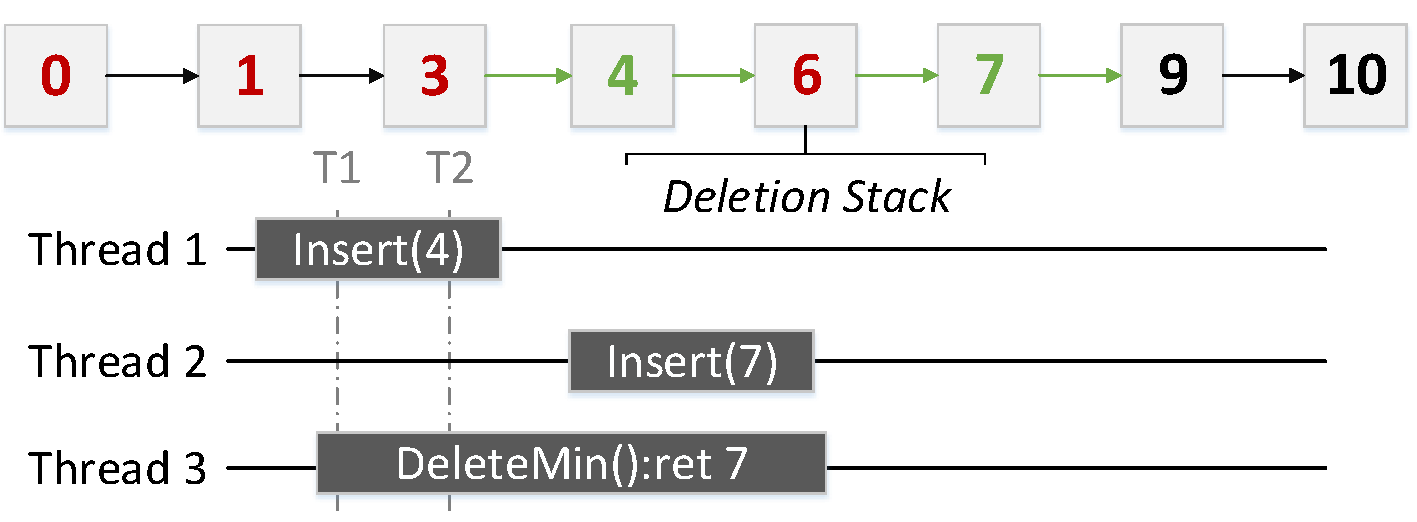
\includegraphics[width=0.82\columnwidth]{./graph/mdlist-3d-quiescent.pdf}
    \caption{Violation of real time order}
    \label{fig:quiescent}
    \vspace{-0.1in}
\end{figure}

However, concurrent execution of \textsc{DeleteMin} and \textsc{Insert} operations may violate the real time ordering required quiescent consistency.
Fig.~\ref{fig:quiescent} shows a such example.
Thread 1 finishes its insertion before thread 2 starts it insertion, but thread 3, which concurrently executes \textsc{DeleteMin}, returns 7 because it reads the deletion stack at $T1$ before thread 1 is able to update the stack at $T2$.
This is because only those nodes $\{n|n \notin M_i\}$ are reachable from $stack_i$ .
At the beginning of the \textsc{DeleteMin} operation, the deletion stack is read once on line~\algref{alg:deletemin}{l:readstack}.
The subsequent traversal will not be aware of any unmarked nodes removed from $M$.

One method of designing a linearizable algorithm is the time-stamping mechanism adopted by Shavit and Lotan in~\cite{shavit2000skiplist}, in which each deletion thread returns the minimal undeleted node among those inserted completely before it reads the deletion stack.
After a node is inserted on line~\algref{alg:insert}{l:link}, it acquires a time-stamp.
A deletion thread notes the time at which it reads the stack and only processes nodes with a smaller time-stamp.  
This time-stamping mechanism ensures that the \textsc{DeleteMin} operations see a consistent abstract state throughout the search process.

%\subsection{Relaxation}
%Our algorithm is relaxed in the sense that it is quiescently consistent.
%We prefer quiescent consistency over linearizability because it allows for higher level of concurrency.
%The trade-off is that in concurrent executions without any quiescence the order in which method calls take effect may be undefined.
%Now we consider the execution of the \textsc{FinishPurging} function.

%\begin{lemma}
    %Purge does not change the abstract state $P$.
%\end{lemma}
%\begin{proof}
    %Note that in Algorithm~\ref{alg:purge}, $L$ does not change because no new node is inserted; $M$ does not change because the deletion stack is not modified; $S$ does not change because no deletion flag is marked.
%\end{proof}

%\begin{theorem} \label{th:bound}
    %Let $key_{prg}$ denote the key of the last $prg$ node in Algorithm~\ref{alg:purge}.
    %Without quiescence, a successful \textsc{DeleteMin} operation either returns $n \in P : \forall n' \in P,\;n.key < n'.key$ or $n \in P : n.key < key_{prg}$.
%\end{theorem}
%\begin{proof}
    %The purge algorithm creates a new head node while keeping the old head, thus the ordering relation between two set of nodes $Q=\{n|n\in L_i \land n.key \le key_{prg}\}$ and $Q'=\{n'|n' \in L_{i+1} \land n'.key \le key_{prg}\}$ is not defined.
%The relaxation takes place when \textsc{Insert} operations overlap with \textsc{Purge} because new nodes can be inserted into either set depending on when the insertion starts.
%If there are quiescent periods between insertions and purges, all new nodes are inserted into $Q'$, which implies $Q \subseteq S$.
%Otherwise, $\exists n\in Q, n' \in Q' : n \notin S \land n' \notin S \land n.key > n'.key$.
%When the \textsc{DeleteMin} operation switches to the new head on line~\algref{alg:deletemin}{l:switchhead} the strict ordering property is temporarily relaxed.
%\end{proof}

%We define the bound of the relaxation by the number of minimal nodes that might be skipped by \textsc{DeleteMin} operations.
%According to Theorem~\ref{th:bound}, the exact upper bound of the relaxation is generally undetermined because it depends on the key of the last purged nodes. 
%However, if the distribution of keys is known beforehand, we could set the purge threshold based on a fixed key, which in turn gives a fixed upper bound.

\begin{figure*}[t]
    \begin{subfigure}{0.33\textwidth}
        \centering
        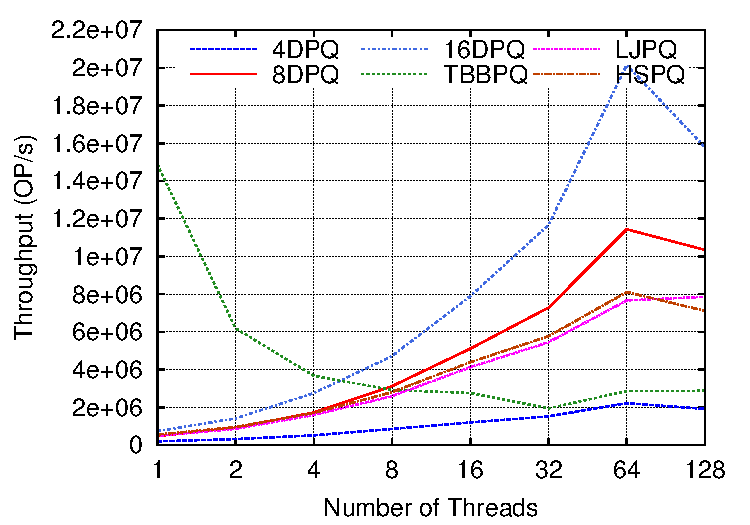
\includegraphics[width=1\columnwidth]{./data/amd100insertion.pdf}
        \caption{NUMA System: 100\% \textsc{Insert}}
        \label{fig:100ins}
    \end{subfigure}
    \hfill
    \begin{subfigure}{0.33\textwidth}
        \centering
        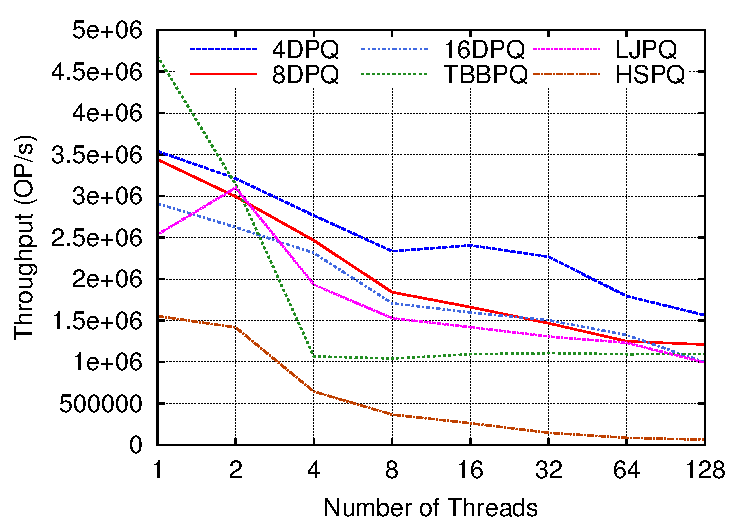
\includegraphics[width=1\columnwidth]{./data/amd0insertion.pdf}
        \caption{NUMA System: 100\% \textsc{DeleteMin}}
        \label{fig:0ins}
    \end{subfigure}
    \hfill
    \begin{subfigure}{0.33\textwidth}
        \centering
        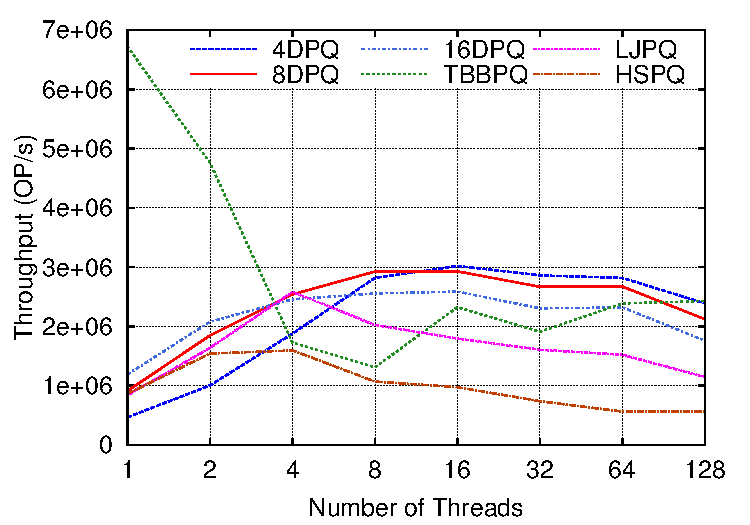
\includegraphics[width=1\columnwidth]{./data/amd50insertion.pdf}
        \caption{NUMA System: 50\% \textsc{Insert}}
        \label{fig:50ins}
    \end{subfigure}
    \begin{subfigure}{0.33\textwidth}
        \centering
        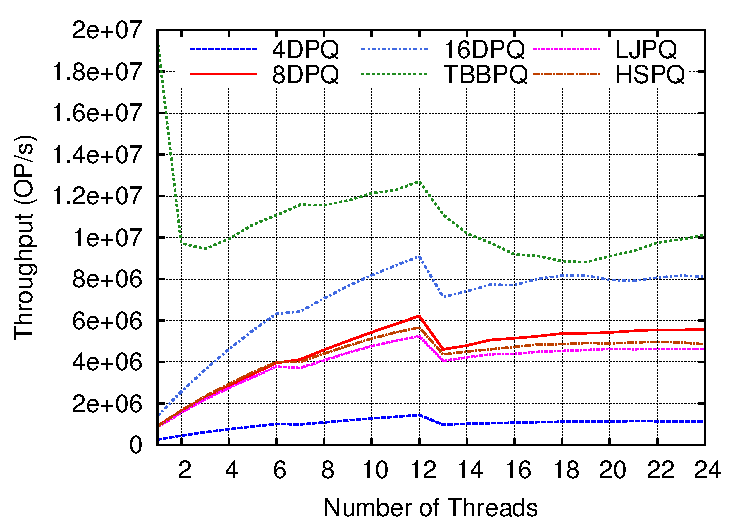
\includegraphics[width=1\columnwidth]{./data/intel100insertion.pdf}
        \caption{SMP System: 100\% \textsc{Insert}}
        \label{fig:100insintel}
    \end{subfigure}
    \hfill
    \begin{subfigure}{0.33\textwidth}
        \centering
        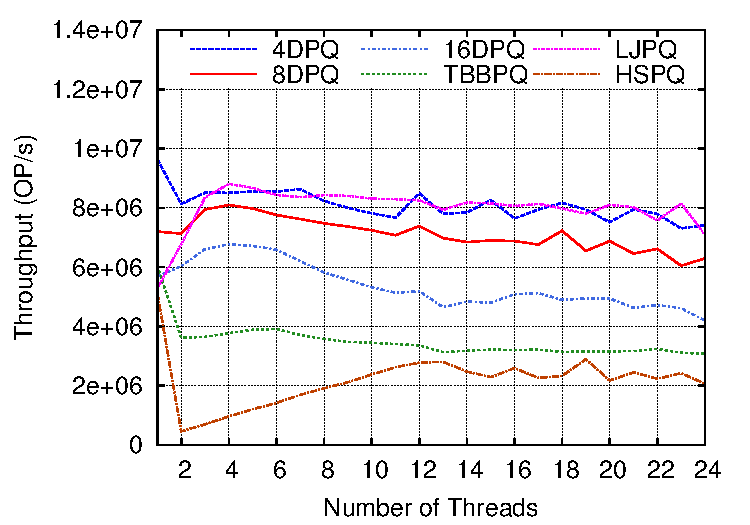
\includegraphics[width=1\columnwidth]{./data/intel0insertion.pdf}
        \caption{SMP System: 100\% \textsc{DeleteMin}}
        \label{fig:0insintel}
    \end{subfigure}
    \hfill
    \begin{subfigure}{0.33\textwidth}
        \centering
        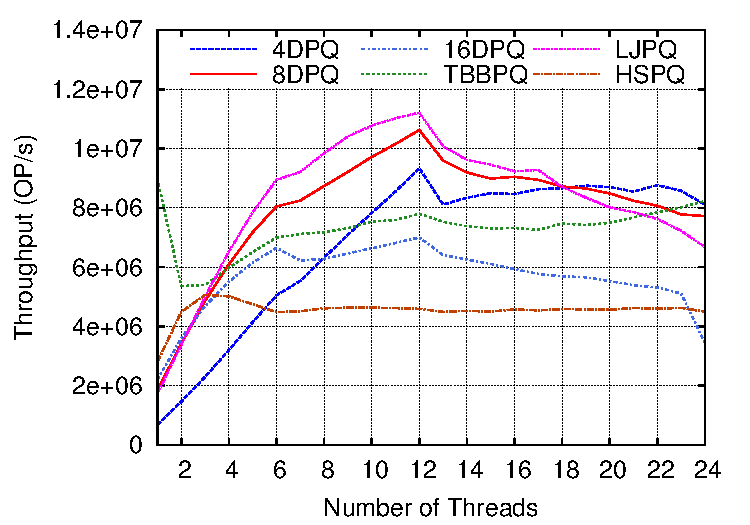
\includegraphics[width=1\columnwidth]{./data/intel50insertion.pdf}
        \caption{SMP System: 50\% \textsc{Insert}}
        \label{fig:50insintel}
    \end{subfigure}
        %\hfill
    %\begin{subfigure}{0.33\textwidth}
        %\centering
        %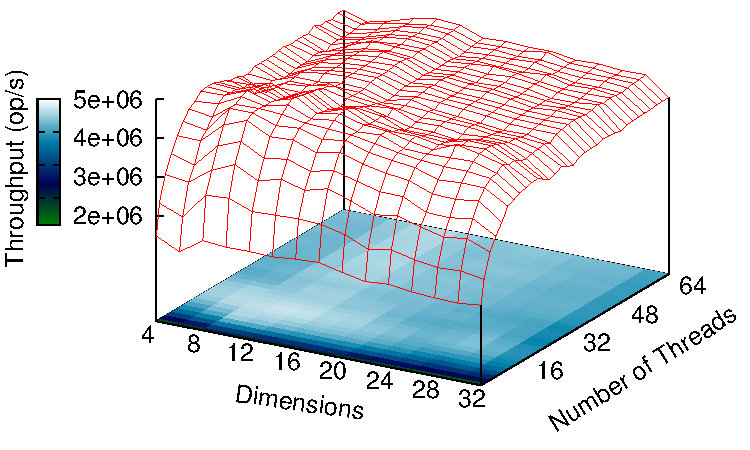
\includegraphics[width=1\columnwidth]{./data/amdsweep75insert.pdf}
        %\caption{Dimensionality and Performance}
        %\label{fig:sweep}
    %\end{subfigure}
    \caption{Throughput of the Priority Queues (MDPQs are named by their dimensionality, e.g. 8DPQ is an MDPQ with 8 dimensions)}
    \label{fig:throughput}
    \vspace{-0.2in}
\end{figure*}


\subsection{Lock Freedom}
Our algorithm is lock-free because it guarantee that for every possibly execution scenario, at least one thread makes progress.
We prove this by examining unbounded loops in all possible execution paths, which can delay the termination of the operations.
\begin{lemma} \label{lmm:finitestep}
    \textsc{FinishInserting} (Algorithm~\ref{alg:adoption}) and \textsc{Purge} (Algorithm~\ref{alg:purge}) complete in finite steps.
\end{lemma}
\begin{proof}
    We observe that \textsc{FinishInserting} does not contain unbounded loop.
    For \textsc{Purge}, the \texttt{repeat} loops on line~\algref{alg:purge}{l:prgwhile} are subject to fail and retry when another insertion thread concurrently updates $pvt.child[i]$.
    The number of retries is bounded by $\sqrt[D]{N}$, which is the maximum number of nodes in each dimension.
    The \texttt{for} loop (line~\algref{alg:purge}{l:prgfor}) is also unbounded.
    According to Invariant~\ref{inv:reachability}, the purged node can always be reached from the head through a sequence of child pointers and the number of reties is bounded by $D \sqrt[D]{N}$.
\end{proof}

\begin{theorem}
    \textsc{Insert} and \textsc{DeleteMin} operations are lock-free.
\end{theorem}
\begin{proof}
    Note that all shared variables are concurrently modified by CAS operations, and the CAS-based unbounded loops (line~\algref{alg:insert}{l:link}, ~\algref{alg:deletemin}{l:delcas}, and ~\algref{alg:rewind}{l:rewindcas}), only retry when a CAS operation fails.
    This means that for any subsequent retry, there must be one CAS that succeeded, which caused the termination of the loop.
    All reads of child pointer are preceded by \textsc{FinishInserting}, which completes child adoption in finite steps to ensure consistency.
    Furthermore, our implementation does not contain cyclic dependencies between CAS-based loops, which means that the corresponding operation will progress.
\end{proof}

\section{Experimental Evaluation}
\label{sec:experiment}

We compare the performance of our algorithm (MDPQ) against Intel TBB's concurrent priority (TBBPQ)~\cite{reinders2007intel}, Linden and Jonsson's linearizable priority queue (LJPQ)~\cite{linden2013skiplist}, and Herlihy and Shavit's quiescently consistent priority queue (HSPQ)~\cite{herlihy2012art}.
Intel TBB is an established industry standard concurrent library.
TBBPQ is based on an array-based heap and employs a dedicated aggregator thread to perform all operations.
It is not lock-free because a halting aggregator thread prevents system wide progress.
LJPQ is the best available linearizable priority queue that minimizes contention on the head node.
HSPQ shares the same correctness guarantee as our algorithm.
Both LJPQ and HSPQ are built on top of Fraser's~\cite{fraser2004practical} state of the art lock-free skiplist implementation and use the epoch-based garbage collection.
TBBPQ allocates contiguous memory chunks with growing capacity but never free them until the termination of the object.
For fair comparison of the algorithm themselves, we disable memory reclamation for all approaches and do not use any back-off strategies.
%but use thread-caching malloc~\cite{ghemawat2009tcmalloc} as a scalable alternative to the standard library malloc.
We employ a micro-benchmark to evaluate the performance of these approaches for uniformly distributed unique 32-bit keys.
This canonical evaluation method~\cite{harris2001pragmatic,shavit2000skiplist,linden2013skiplist,sundell2005fast} consists of a tight loop that randomly chooses to perform either an \textsc{Insert} or a \textsc{DeleteMin} operation. 
Each thread performs one million operations and we take the average from three runs.
The tests are conducted on a 64-core NUMA system (4 AMD opteron 6272 CPUs with 16 cores per chip @2.1 GHz) and a 12-core SMP system (1 Intel Xeon X5670 CPU with hyper-threading @2.9GHz). 
Both the micro-benchmark and the priority queue implementations\footnote{Source code can be requested from \url{http://cse.eecs.ucf.edu/request.php?project=13}} are compiled with GCC 4.7 with level three optimizations.

\begin{figure*}[t]
    \begin{subfigure}{0.33\textwidth}
        \centering
        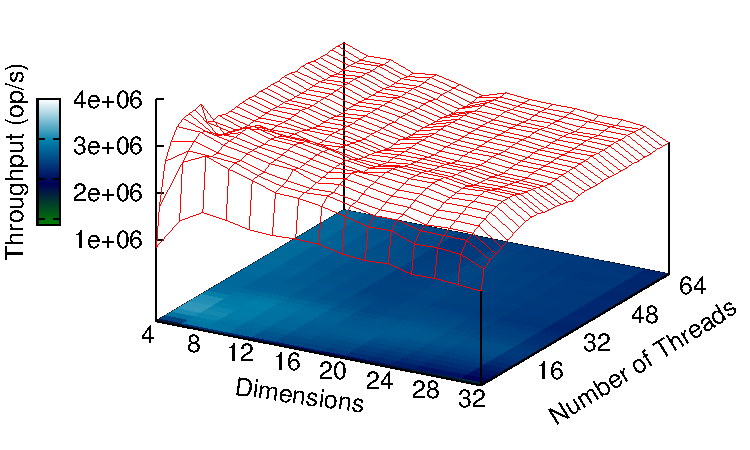
\includegraphics[width=1\columnwidth]{./data/amdsweep50insert.pdf}
        \caption{NUMA System: 50\% \textsc{Insert}}
        \label{fig:dimsweep50}
    \end{subfigure}
    \hfill
    \begin{subfigure}{0.33\textwidth}
        \centering
        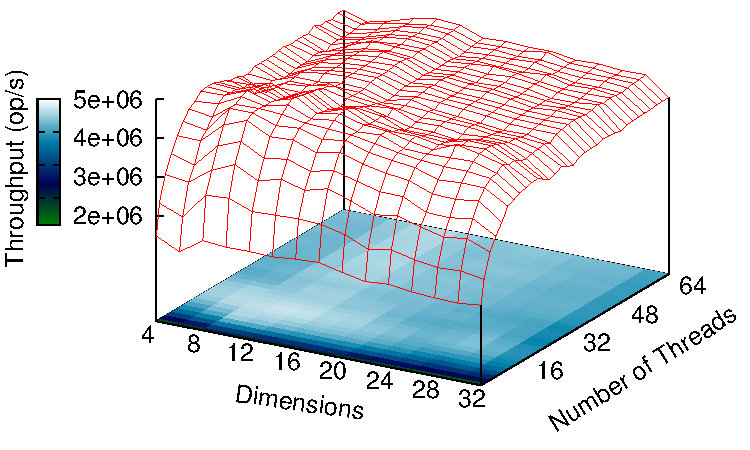
\includegraphics[width=1\columnwidth]{./data/amdsweep75insert.pdf}
        \caption{NUMA System: 75\% \textsc{Insert}}
        \label{fig:dimsweep75}
    \end{subfigure}
    \hfill
    \begin{subfigure}{0.33\textwidth}
        \centering
        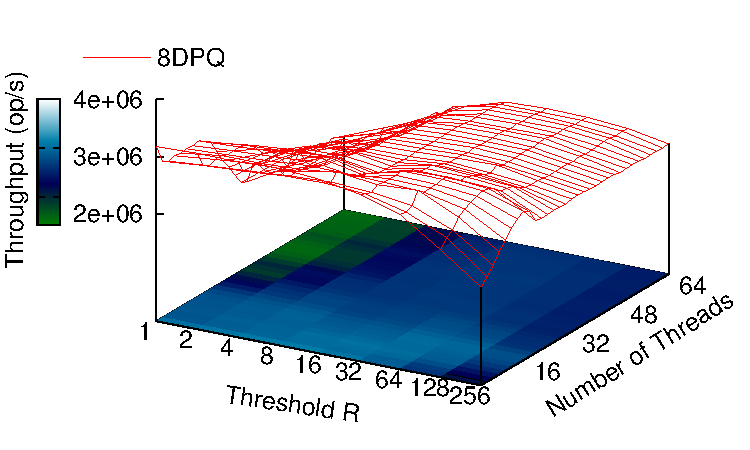
\includegraphics[width=1\columnwidth]{./data/amdsweepprg50insert.pdf}
        \vspace{-0.17in}
        \caption{NUMA System: 50\% \textsc{Insert}}
        \label{fig:prgsweep}
    \end{subfigure}
    \caption{Performance Impact of Dimensionality and Purge Threshold}
    \label{fig:sweep}
    \vspace{-0.2in}
\end{figure*}

\subsection{Throughput}
Fig.~\ref{fig:100ins},~\ref{fig:0ins} and~\ref{fig:50ins} illustrate the throughput of the algorithms on the NUMA system.
The $y$-axis represents the throughput measured by \emph{operation per second}, and the $x$-axis represents the number of threads.
In Fig.~\ref{fig:100ins}, threads perform solely \textsc{Insert} operations.
We observe that the skiplist-based and MDList-based approaches explore fine-grained parallelism and exhibit similar scalability trends.
The throughput increases linearly until 16 threads, and continues to increase at a slower pace until 64 threads.
Because executions beyond 16 threads span across multiple chips, the performance growth is slightly reduced due to the cost of remote memory accesses.
The executions are no longer fully concurrent beyond 64 threads, thus the overall throughput is capped and may even reduce due to context switching overhead.
The performance of LJPQ are on par with HSPQ because they employs identical skiplist insertion algorithms.
Our priority queue based on an 8DList (8DPQ) achieves a $24\%$ speedup over LJPQ on 16 threads and a further $50\%$ speedup on 64 threads.
Each insertion in MDPQ modifies at most two consecutive nodes, incurring less remote memory access than skiplist-based approaches.
When we increase the dimensionality of MDPQ to 16, we obtain on average a $50\%$ throughput gain over 8DPQ.
A 16DPQ contains at most 4 nodes in each dimension.
In order to reach the target position the search operation traverses a maximum of 64 nodes comparing to 128 nodes in a 8DPQ.
Further increases in dimensionality can result in diminishing returns for concurrent \textsc{Insert}.
The growing number of child pointers causes synchronization overhead that cancels the benefit of having less nodes in each dimension.
TBBPQ, on the other hand, exhibits reduced throughput when increasing the number of threads.
Its heap-based structure achieves high throughput on a single thread, but the aggregator effectively serializes all operations and limits the throughput in concurrent executions.

Fig.~\ref{fig:0ins} shows the results for \textsc{DeleteMin} operations.
We fill the data structures with one million elements and measure the time it takes to dequeue them.
The overall throughput decreases as the number of threads increases, which matches the observation that \textsc{DeleteMin} is the sequential bottleneck of a priority queue algorithm.
Throughput of HSPQ drops significantly because it initiates physical deletion for every logically deleted node.
The physical deletion constantly swings pointers which causes heavy content on the head node.
8DPQ and LJPQ achieve comparable performance because they both employ batch physical deletion, which reduces the total number of pointer updates.
4DPQ outperforms LJPQ by $50\%$ starting from 16 threads because the number of pointers, which the deletion needs to update, reduces as dimensionality decreases.
TBBPQ is able to keep a constant throughput starting from 4 threads.
As the \textsc{DeleteMin} operation is intrinsically sequential, having a dedicated aggregator helps relieve contention by allowing other threads to wait while a single thread performs the update.
%However, since it does not explore fine-grained parallelism, its throughput is still below average.

We show the results where threads randomly choose operations with a distribution of 50\% \textsc{Insert} and 50\% \textsc{DeleteMin} in Fig.~\ref{fig:50ins}.
As the level of concurrency increases, the overall throughput peaks at some point where the executions strike a balance between the increasing throughput of \textsc{Insert} and the decreasing throughput of \textsc{DeleteMin}.
8DPQ exhibits the best overall throughput, outperforming LJPQ by $50\%$ starting from 8 threads.
Our algorithm allows insertion of new nodes into a position before a logically deleted node.
The concurrent executions of \textsc{Insert} and \textsc{DeleteMin} guarantees quiescent consistency, which is relaxed compared to linearizability.
This helps improve throughput over Linden's logical deletion scheme where deletion threads cannot proceed past an ongoing insertion~\cite{linden2013skiplist}.
4DPQ achieves about $10\%$ speedup over 8DPQ on 64 and 128 threads at the price of being slower when the number of threads is low. 

Fig.~\ref{fig:100insintel} ~\ref{fig:0insintel} and~\ref{fig:50ins} show the throughput of the algorithms on the SMP system.
In Fig.~\ref{fig:100insintel} MDList-based and Skiplist-based approaches exhibits similar scalability trend as on the NUMA system, with 16DPQ outperform LJPQ by as much as of $70\%$ starting from 10 threads.
TBBPQ performs well its contiguous heap structure is specifically optimized for Intel chips, which provides larger cache than the AMD chip.
In Fig.~\ref{fig:0insintel} 4DPQ and LJPQ perform equally well.
In Fig.~\ref{fig:50insintel} 8DPQ and LJPQ achieve comparable throughput, obtaining $30\%$ speedup over TBBPQ and $50\%$ over HSPQ with 12 threads.
Executions beyond 12 threads are preemptive, and the overhead of context switching leads to a reduction of 8DPQ and LJPQ's throughput.
%The SMP system contains a single Intel CPU, which has a shorter memory latency than the AMD system.

\subsection{Tuning}
In Fig.~\ref{fig:dimsweep50} and~\ref{fig:dimsweep75}, we sweep the dimension of MDPQ from 4 to 32 on the NUMA system.
The lighter color on the color coded heat map indicates higher throughput.
In Fig.~\ref{fig:dimsweep50}, we observe the max throughput converges towards 4 dimensions on most scale levels.
In Fig.~\ref{fig:dimsweep75} we increase the number of insertions to create a write-dominated workload.
This is to simulate the typical access pattern of best-first search algorithms, in which a worker thread insert multiple new nodes (search state) upon dequeuing the node with highest priority~\cite{burns2010best}.
On all scale levels, we see that the throughput converges towards 12 dimensions.
This implies that if the access pattern of the user application is taken into account the performance of MDPQ can be optimized  without knowing how many threads are going to access the data structure.
The dimensionality sweep also reveals that the overall throughput is capped with 16 threads.
This implies that the algorithms with inherent sequential semantics, such the \textsc{DeleteMin} operation, pose scalability challenges for NUMA systems.

In Fig.~\ref{fig:prgsweep} we evaluate the performance impact of purge threshold $R$.
We observe that the maximum throughput converges towards $32 \le R \le 64$.
Note that $R \le 4$ greatly limits the throughput under high concurrency.
Generally, smaller $R$ values cause more frequent purges, which incurs overhead. 
Larger $R$ values result in more undeleted nodes, which slows down logical deletion. 
Good $R$ values strike a balance between these two scenarios.

In summary, MDPQ provides scalable performance under high concurrency.
The locality of its operations makes it suitable for NUMA architectures where remote memory access incurs considerable performance penalties.
On an SMP system with low levels of concurrency, MDPQ performs better than the state of the art skiplist-based approaches under write-dominate workload and equally well under mixed workload.
MDPQ can also adapt to different workload: a high-dimensional priority queue behaves more like a tree and speeds up insertions; a low-dimensional priority queue behaves more like a linked list and speeds up deletions.

\vspace{-0.1in}
\section{Conclusion}
\label{sec:conclusion}
In this paper, we introduced a lock-free priority queue design based on a novel multi-dimensional list.
The proposed MDList guarantees logarithmic worst-case search time by mapping keys into high dimensional coordinates.
We exploited spatial locality to increase the throughput of the \textsc{Insert} operation, and adopted quiescent consistency to address the sequential bottleneck of the \textsc{DeleteMin} operation.
When compared to the best available skiplist-based and heap-based algorithms, our algorithm achieved an average of $50\%$ speedup on a 64-core NUMA system.
We plan to further evaluate our approach on SMP system with more cores, such as Intel Xeon Phi, to verify potential performance gain under high concurrency.
The performance of an MDList-based data structure can be tailored to different access patterns by changing its dimensionality.
This implies the possibility of a workload aware algorithm.
Furthermore, an MDList provides a scalable alternative to skiplists and search trees, which opens up opportunities for implementing other multiprocessor data structures, such as dictionaries and sparse vectors. 

\bibliographystyle{abbrv}
\bibliography{citation}

\begin{IEEEbiography}[{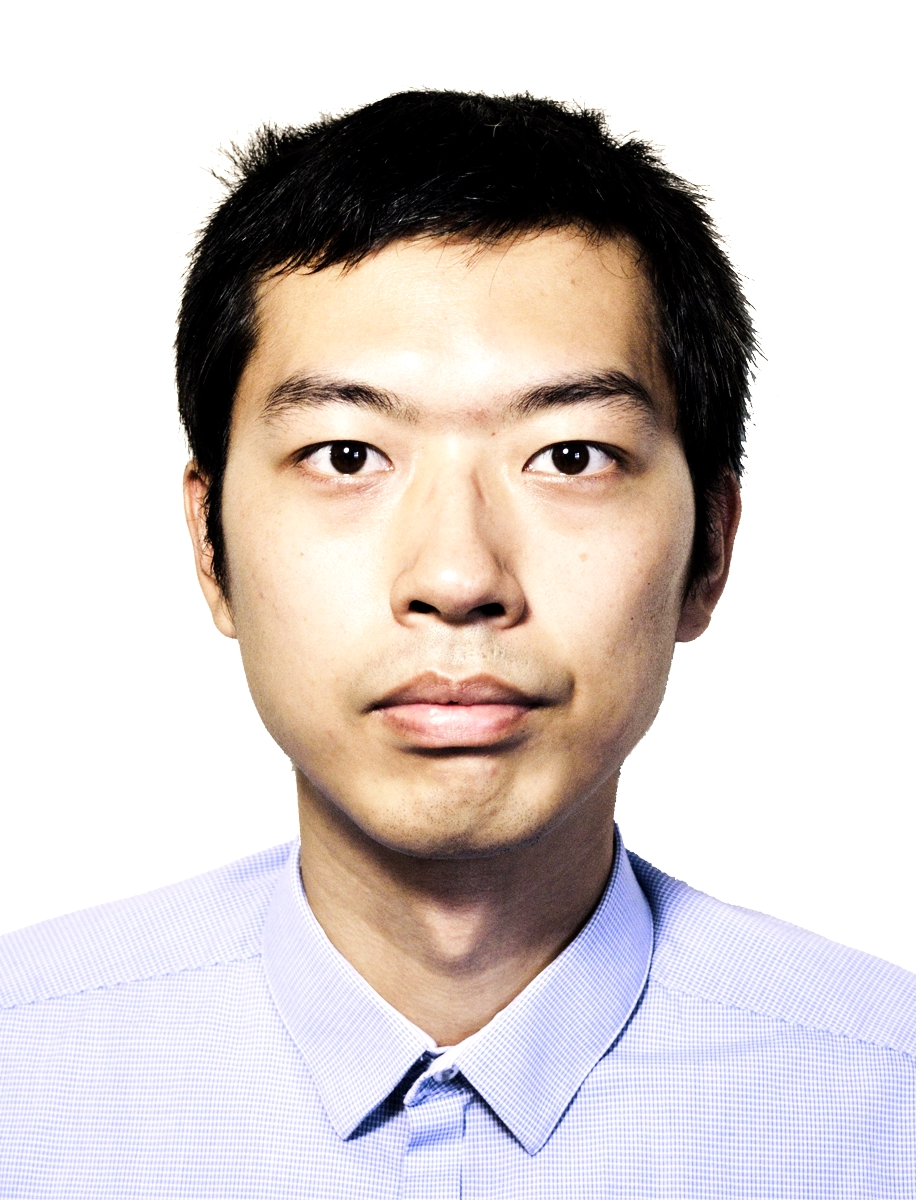
\includegraphics[width=1in,height=1.25in,clip,keepaspectratio]{./graph/deli_bio.png}}]{Deli Zhang}
Deli Zhang is a Ph.D. student at the EECS Department at the University of Central Florida. He is also a research assistant in the Computer Software Engineering - Scalable and Secure Systems Lab at UCF. His research interests include developing non-blocking data structures and algorithms, applying non-blocking synchronization in existing performance critical applications.
\end{IEEEbiography}
%\vspace{-0.4in}
\begin{IEEEbiography}[{
\includegraphics[width=1in,height=1.25in,clip,keepaspectratio]{./graph/damian_bio.png}}]{Damian Dechev}
Dr. Damian Dechev is an Assistant Professor at the EECS Department at the University of Central Florida and the founder of the Computer Software Engineering - Scalable and Secure Systems Lab at UCF. He specializes in the design of scalable multiprocessor data structures and algorithms and has applied them in the design of real-time embedded space systems at NASA JPL and the HPC data-intensive applications at Sandia National Labs. 
%In the past four years Dr. Dechev's research in multiprocessor algorithm design has been supported by grants from the National Science Foundation, Sandia National Laboratories, and the Department of Energy.
\end{IEEEbiography}

\vfill

\end{document}
